\documentclass[12pt,a4paper]{article}

% Packages
\usepackage[utf8]{inputenc}
\usepackage[T1]{fontenc}
\usepackage{geometry}
\usepackage{graphicx}
\usepackage{booktabs}
\usepackage{amsmath}
\usepackage{amssymb}
\usepackage{hyperref}
\usepackage{natbib}
\usepackage{float}
\usepackage{caption}
\usepackage{subcaption}
\usepackage{xcolor}
\usepackage{array}
\usepackage{multirow}
\usepackage{fancyhdr}
\usepackage{setspace}

% Page geometry
\geometry{
    left=2.5cm,
    right=2.5cm,
    top=2.5cm,
    bottom=2.5cm
}

% Line spacing
\onehalfspacing

% Header/Footer
\pagestyle{fancy}
\fancyhf{}
\fancyhead[L]{\small Benford's Law Analysis}
\fancyhead[R]{\small \thepage}
\renewcommand{\headrulewidth}{0.4pt}

% Colors for risk levels
\definecolor{lowrisk}{RGB}{40, 167, 69}
\definecolor{mediumrisk}{RGB}{255, 193, 7}
\definecolor{highrisk}{RGB}{253, 126, 20}
\definecolor{criticalrisk}{RGB}{220, 53, 69}

% Hyperref setup
\hypersetup{
    colorlinks=true,
    linkcolor=blue,
    citecolor=blue,
    urlcolor=blue
}

% Graphics path
\graphicspath{{figures/}}

\begin{document}

% Title Page
\begin{titlepage}
    \centering
    \vspace*{2cm}

    {\LARGE \textbf{Detecting Financial Irregularities Using Benford's Law:}}\\[0.5cm]
    {\LARGE \textbf{An Analysis of 442 S\&P 500 Companies}}\\[2cm]

    {\large Diploma Thesis}\\[1cm]

    \vfill

    {\large
    \textbf{Analysis Period:} 2014--2024\\[0.3cm]
    \textbf{Companies Analyzed:} 442\\[0.3cm]
    \textbf{Data Source:} SEC EDGAR Financial Statement Data Sets\\[1cm]
    }

    \vfill

    {\large January 2026}
\end{titlepage}

% Abstract
\newpage
\begin{abstract}
This thesis applies Benford's Law to analyze the first-digit distribution of financial statement numbers from 442 publicly traded U.S. companies over an 11-year period (2014--2024). Using data from the Securities and Exchange Commission (SEC) EDGAR database, we calculate chi-square statistics, Mean Absolute Deviation (MAD), and Kolmogorov-Smirnov test results for each company-year observation.

Our analysis reveals that \textbf{97.5\% of companies} show statistically significant deviation from Benford's expected distribution ($p < 0.05$), with an average chi-square value of 59.83---nearly four times the critical threshold of 15.507. We identify a notable \textbf{post-2019 structural shift}, with mean chi-square values increasing by 24\% compared to the 2014--2018 period.

Case studies of high-anomaly companies (Shake Shack, Medical Properties Trust) and low-anomaly companies (Oracle, Bank of America) provide insights into factors affecting Benford conformance. Importantly, we find only a \textbf{weak correlation} ($r = 0.03$) between Benford anomalies and stock market performance, suggesting that financial reporting irregularities are not directly predictive of investment returns.

These findings contribute to forensic accounting literature and provide a framework for automated financial statement screening.

\textbf{Keywords:} Benford's Law, forensic accounting, fraud detection, SEC filings, chi-square test, financial statement analysis
\end{abstract}

% Table of Contents
\newpage
\tableofcontents

% Main Content
\newpage
\section{Introduction}

\subsection{Background and Motivation}

Financial statement fraud remains a significant concern for investors, regulators, and auditors worldwide. Traditional audit procedures, while essential, may not detect subtle manipulations in reported figures. Benford's Law offers a powerful statistical tool for identifying anomalous patterns that warrant further investigation.

Benford's Law, also known as the First-Digit Law, describes the frequency distribution of leading digits in many naturally occurring datasets \citep{benford1938}. Contrary to intuition, digits do not appear with equal probability; instead, the digit 1 appears as the first digit approximately 30.1\% of the time, while 9 appears only 4.6\% of the time.

\subsection{Benford's Law: Mathematical Foundation}

The probability of digit $d$ appearing as the first significant digit is given by:

\begin{equation}
P(d) = \log_{10}\left(1 + \frac{1}{d}\right), \quad d \in \{1, 2, ..., 9\}
\end{equation}

This yields the expected distribution shown in Figure~\ref{fig:benford_expected}.

\begin{figure}[H]
    \centering
    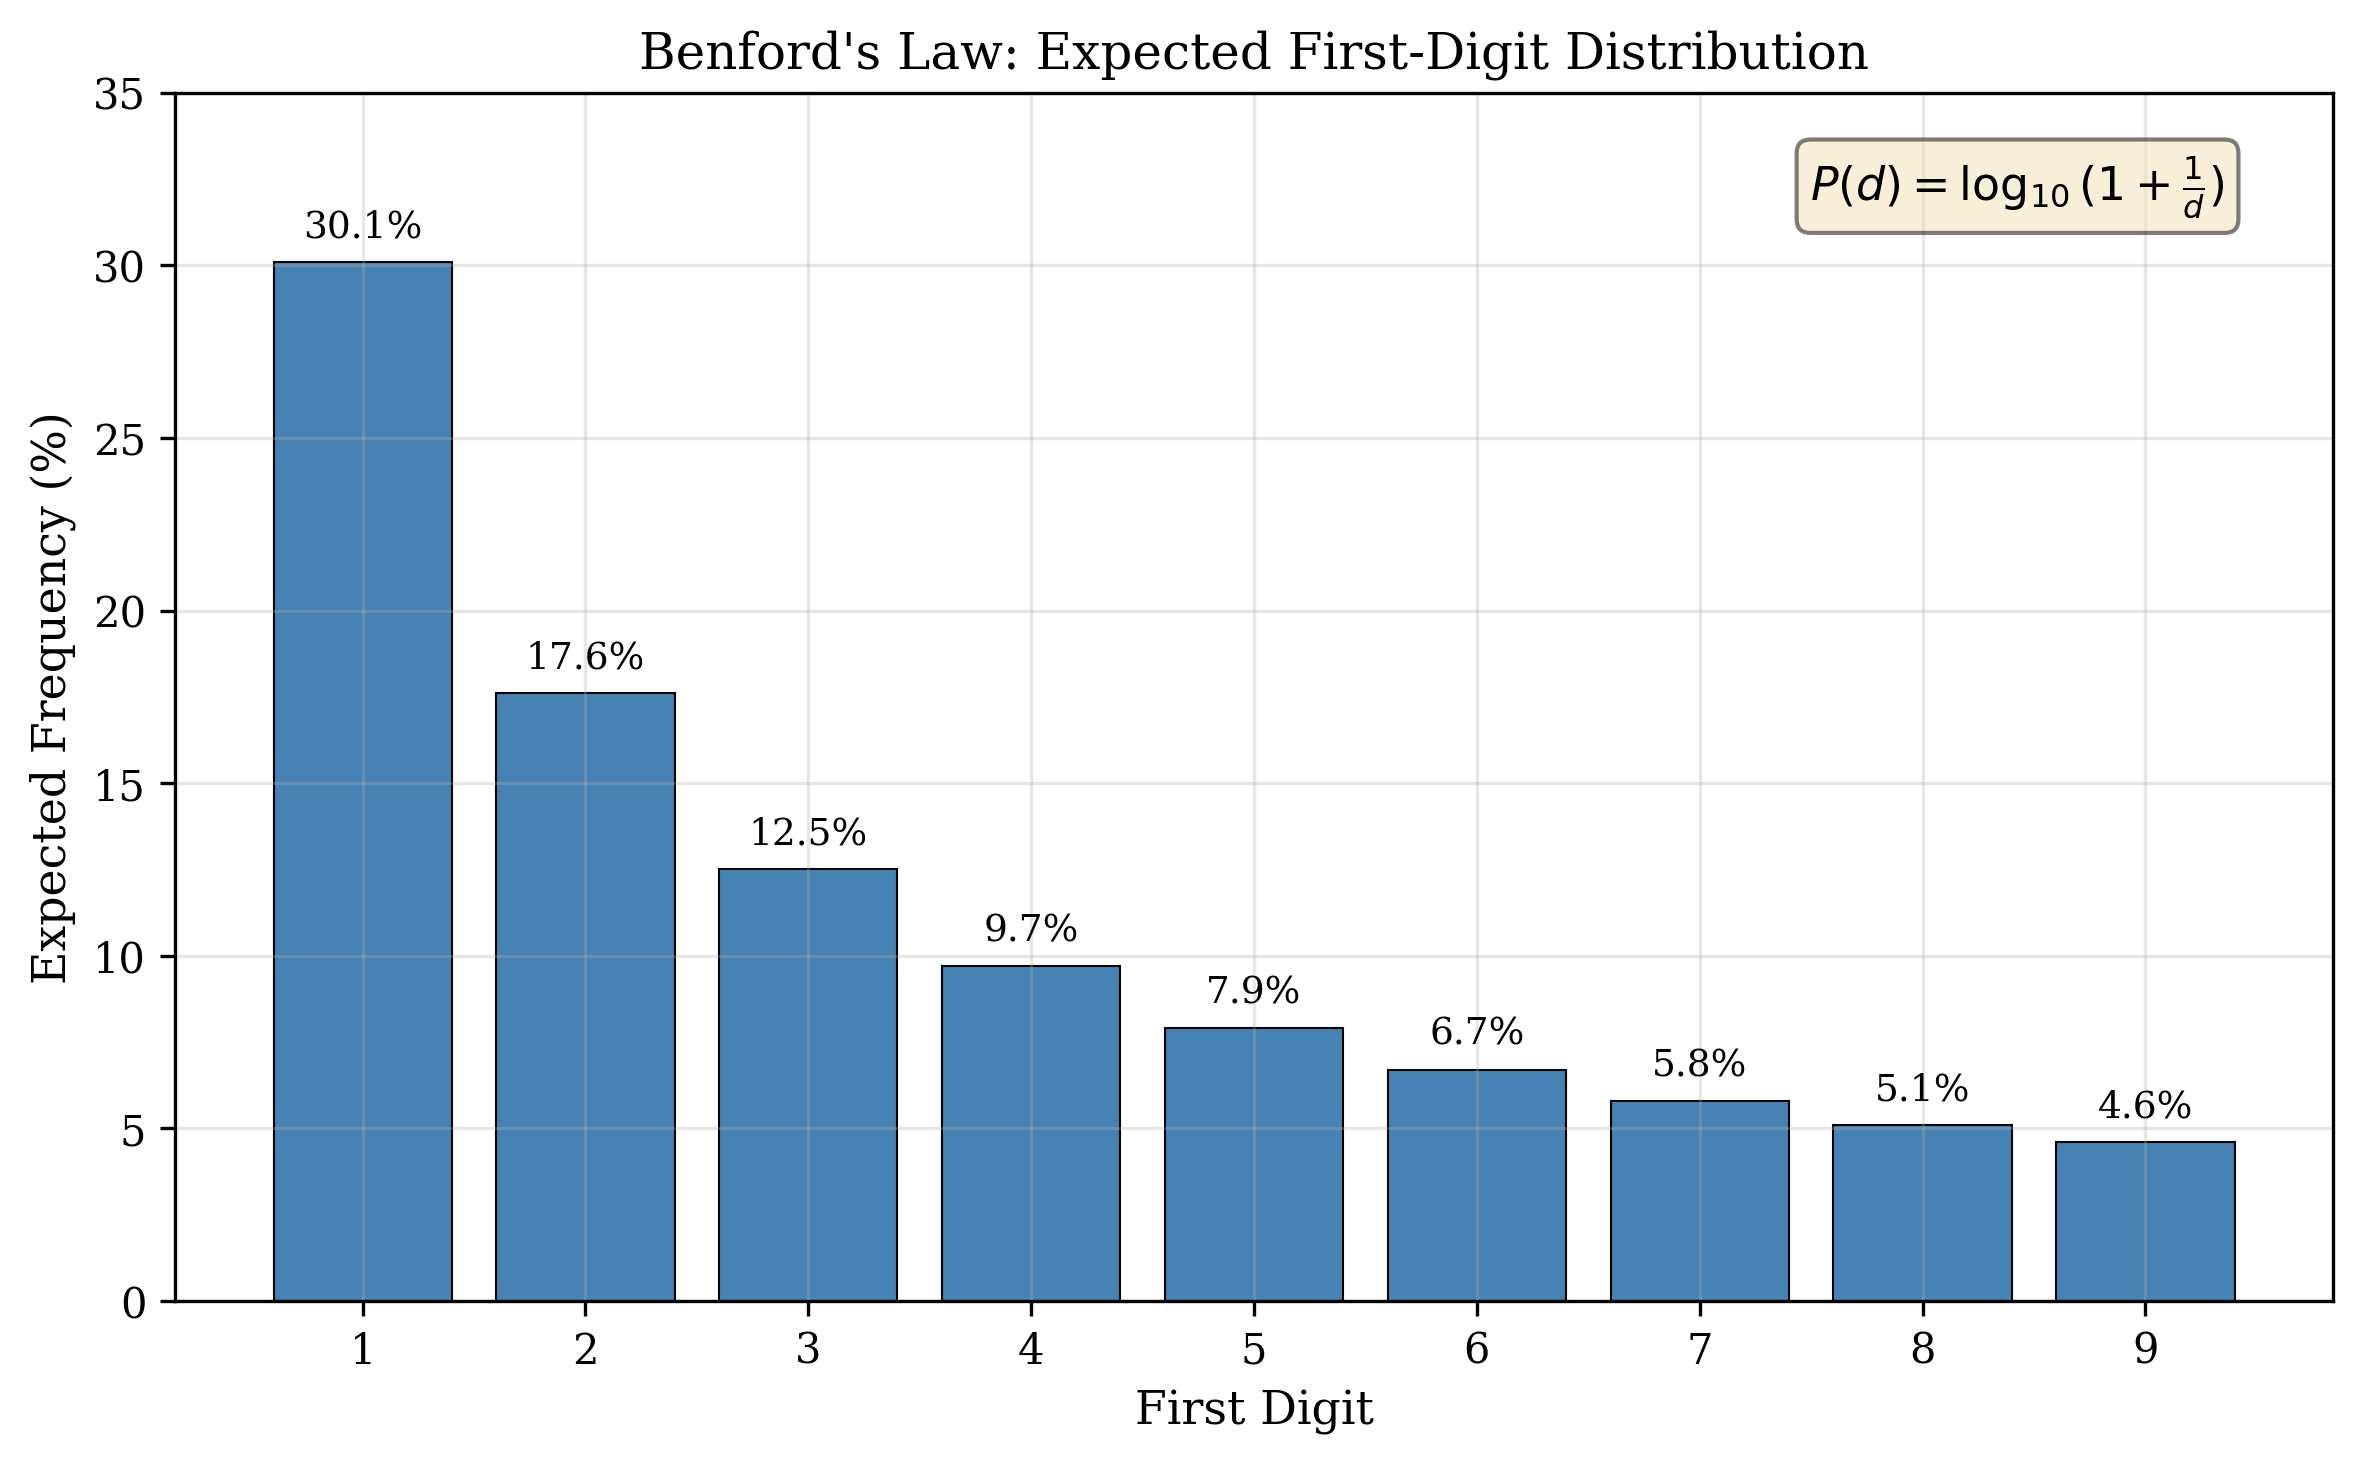
\includegraphics[width=0.85\textwidth]{benford_expected.png}
    \caption{Benford's Law: Expected first-digit distribution. The probability decreases logarithmically from 30.1\% for digit 1 to 4.6\% for digit 9.}
    \label{fig:benford_expected}
\end{figure}

First discovered by astronomer Simon Newcomb in 1881 \citep{newcomb1881} and later independently formulated by physicist Frank Benford \citep{benford1938}, this law has since been proven mathematically under scale and base invariance conditions \citep{hill1995}.

\subsection{Applications in Forensic Accounting}

The application of Benford's Law to accounting data was pioneered by \citet{carslaw1988} and \citet{thomas1989}, who found evidence of earnings manipulation in reported income figures. \citet{nigrini1996, nigrini1999} developed practical methodologies for auditors, establishing threshold values for identifying suspicious deviations.

Key applications include:
\begin{itemize}
    \item Detection of fraudulent financial statements
    \item Tax fraud identification
    \item Election result verification
    \item Scientific data integrity checking
\end{itemize}

\subsection{Research Objectives}

This study aims to:
\begin{enumerate}
    \item Analyze Benford conformance of 442 major U.S. public companies over 11 years
    \item Identify temporal trends and structural changes in financial reporting patterns
    \item Examine the relationship between Benford anomalies and stock market performance
    \item Provide case studies of high and low anomaly companies
\end{enumerate}

\newpage
\section{Methodology}

\subsection{Data Collection}

Financial data was obtained from the SEC EDGAR Financial Statement Data Sets \citep{sec2024}, which provide standardized quarterly filings for all public companies. Our dataset spans:

\begin{itemize}
    \item \textbf{Time Period:} Q1 2014 -- Q4 2024 (44 quarters)
    \item \textbf{Companies:} 442 unique SEC filers
    \item \textbf{Observations:} 4,862 company-year records
\end{itemize}

For each company-year, we extracted all numerical values from financial statements, excluding zero values (which violate Benford's Law assumptions) and taking absolute values of negative figures.

\subsection{Statistical Tests}

We employ four complementary statistical tests to assess Benford conformance:

\subsubsection{Chi-Square Test}

The chi-square goodness-of-fit test compares observed frequencies to Benford's expected distribution:

\begin{equation}
\chi^2 = \sum_{d=1}^{9} \frac{(O_d - E_d)^2}{E_d}
\end{equation}

where $O_d$ is the observed count and $E_d = n \cdot P(d)$ is the expected count for digit $d$.

With 8 degrees of freedom, the critical value at $\alpha = 0.05$ is \textbf{15.507}.

\subsubsection{Mean Absolute Deviation (MAD)}

MAD provides a more interpretable measure of deviation:

\begin{equation}
\text{MAD} = \frac{1}{9} \sum_{d=1}^{9} |O_d\% - E_d\%|
\end{equation}

Following \citet{nigrini2012}, we use these threshold interpretations:

\begin{table}[H]
\centering
\caption{MAD Threshold Interpretations for First-Digit Tests}
\label{tab:mad_thresholds}
\begin{tabular}{lll}
\toprule
\textbf{MAD Range} & \textbf{Interpretation} & \textbf{Risk Level} \\
\midrule
$< 0.006$ & Close conformity & \textcolor{lowrisk}{Low} \\
$0.006 - 0.012$ & Acceptable conformity & \textcolor{lowrisk}{Low} \\
$0.012 - 0.015$ & Marginally acceptable & \textcolor{mediumrisk}{Medium} \\
$> 0.015$ & Nonconformity & \textcolor{highrisk}{High} \\
\bottomrule
\end{tabular}
\end{table}

Note: In our implementation, MAD values are reported as percentages (multiplied by 100), so thresholds become 1.5, 2.5, etc.

\subsubsection{Kolmogorov-Smirnov Test}

The KS test measures the maximum distance between empirical and theoretical cumulative distribution functions \citep{kolmogorov1933}:

\begin{equation}
D = \max_{d} |F_n(d) - F(d)|
\end{equation}

\subsubsection{P-Value}

The p-value from the chi-square test indicates the probability of observing such deviation by chance. Values below 0.05 indicate statistically significant deviation from Benford's Law.

\subsection{Risk Classification}

Companies are classified into risk levels based on average MAD scores:

\begin{table}[H]
\centering
\caption{Risk Classification Criteria}
\label{tab:risk_levels}
\begin{tabular}{llc}
\toprule
\textbf{Risk Level} & \textbf{MAD Range} & \textbf{Color Code} \\
\midrule
Low Risk & MAD $< 1.5$ & \textcolor{lowrisk}{\rule{1cm}{0.3cm}} \\
Medium Risk & $1.5 \leq$ MAD $< 2.5$ & \textcolor{mediumrisk}{\rule{1cm}{0.3cm}} \\
High Risk & $2.5 \leq$ MAD $< 4.0$ & \textcolor{highrisk}{\rule{1cm}{0.3cm}} \\
Critical Risk & MAD $\geq 4.0$ & \textcolor{criticalrisk}{\rule{1cm}{0.3cm}} \\
\bottomrule
\end{tabular}
\end{table}

\newpage
\section{Results}

\subsection{Overall Conformance Rates}

Our analysis reveals widespread deviation from Benford's Law among publicly traded companies:

\begin{itemize}
    \item \textbf{97.5\%} of companies show statistically significant deviation ($p < 0.05$) in at least one year
    \item Average chi-square: \textbf{59.83} (vs. critical value of 15.507)
    \item Average MAD: \textbf{1.83} (indicating general nonconformity)
\end{itemize}

Figure~\ref{fig:mad_histogram} shows the distribution of MAD values across all company-year observations.

\begin{figure}[H]
    \centering
    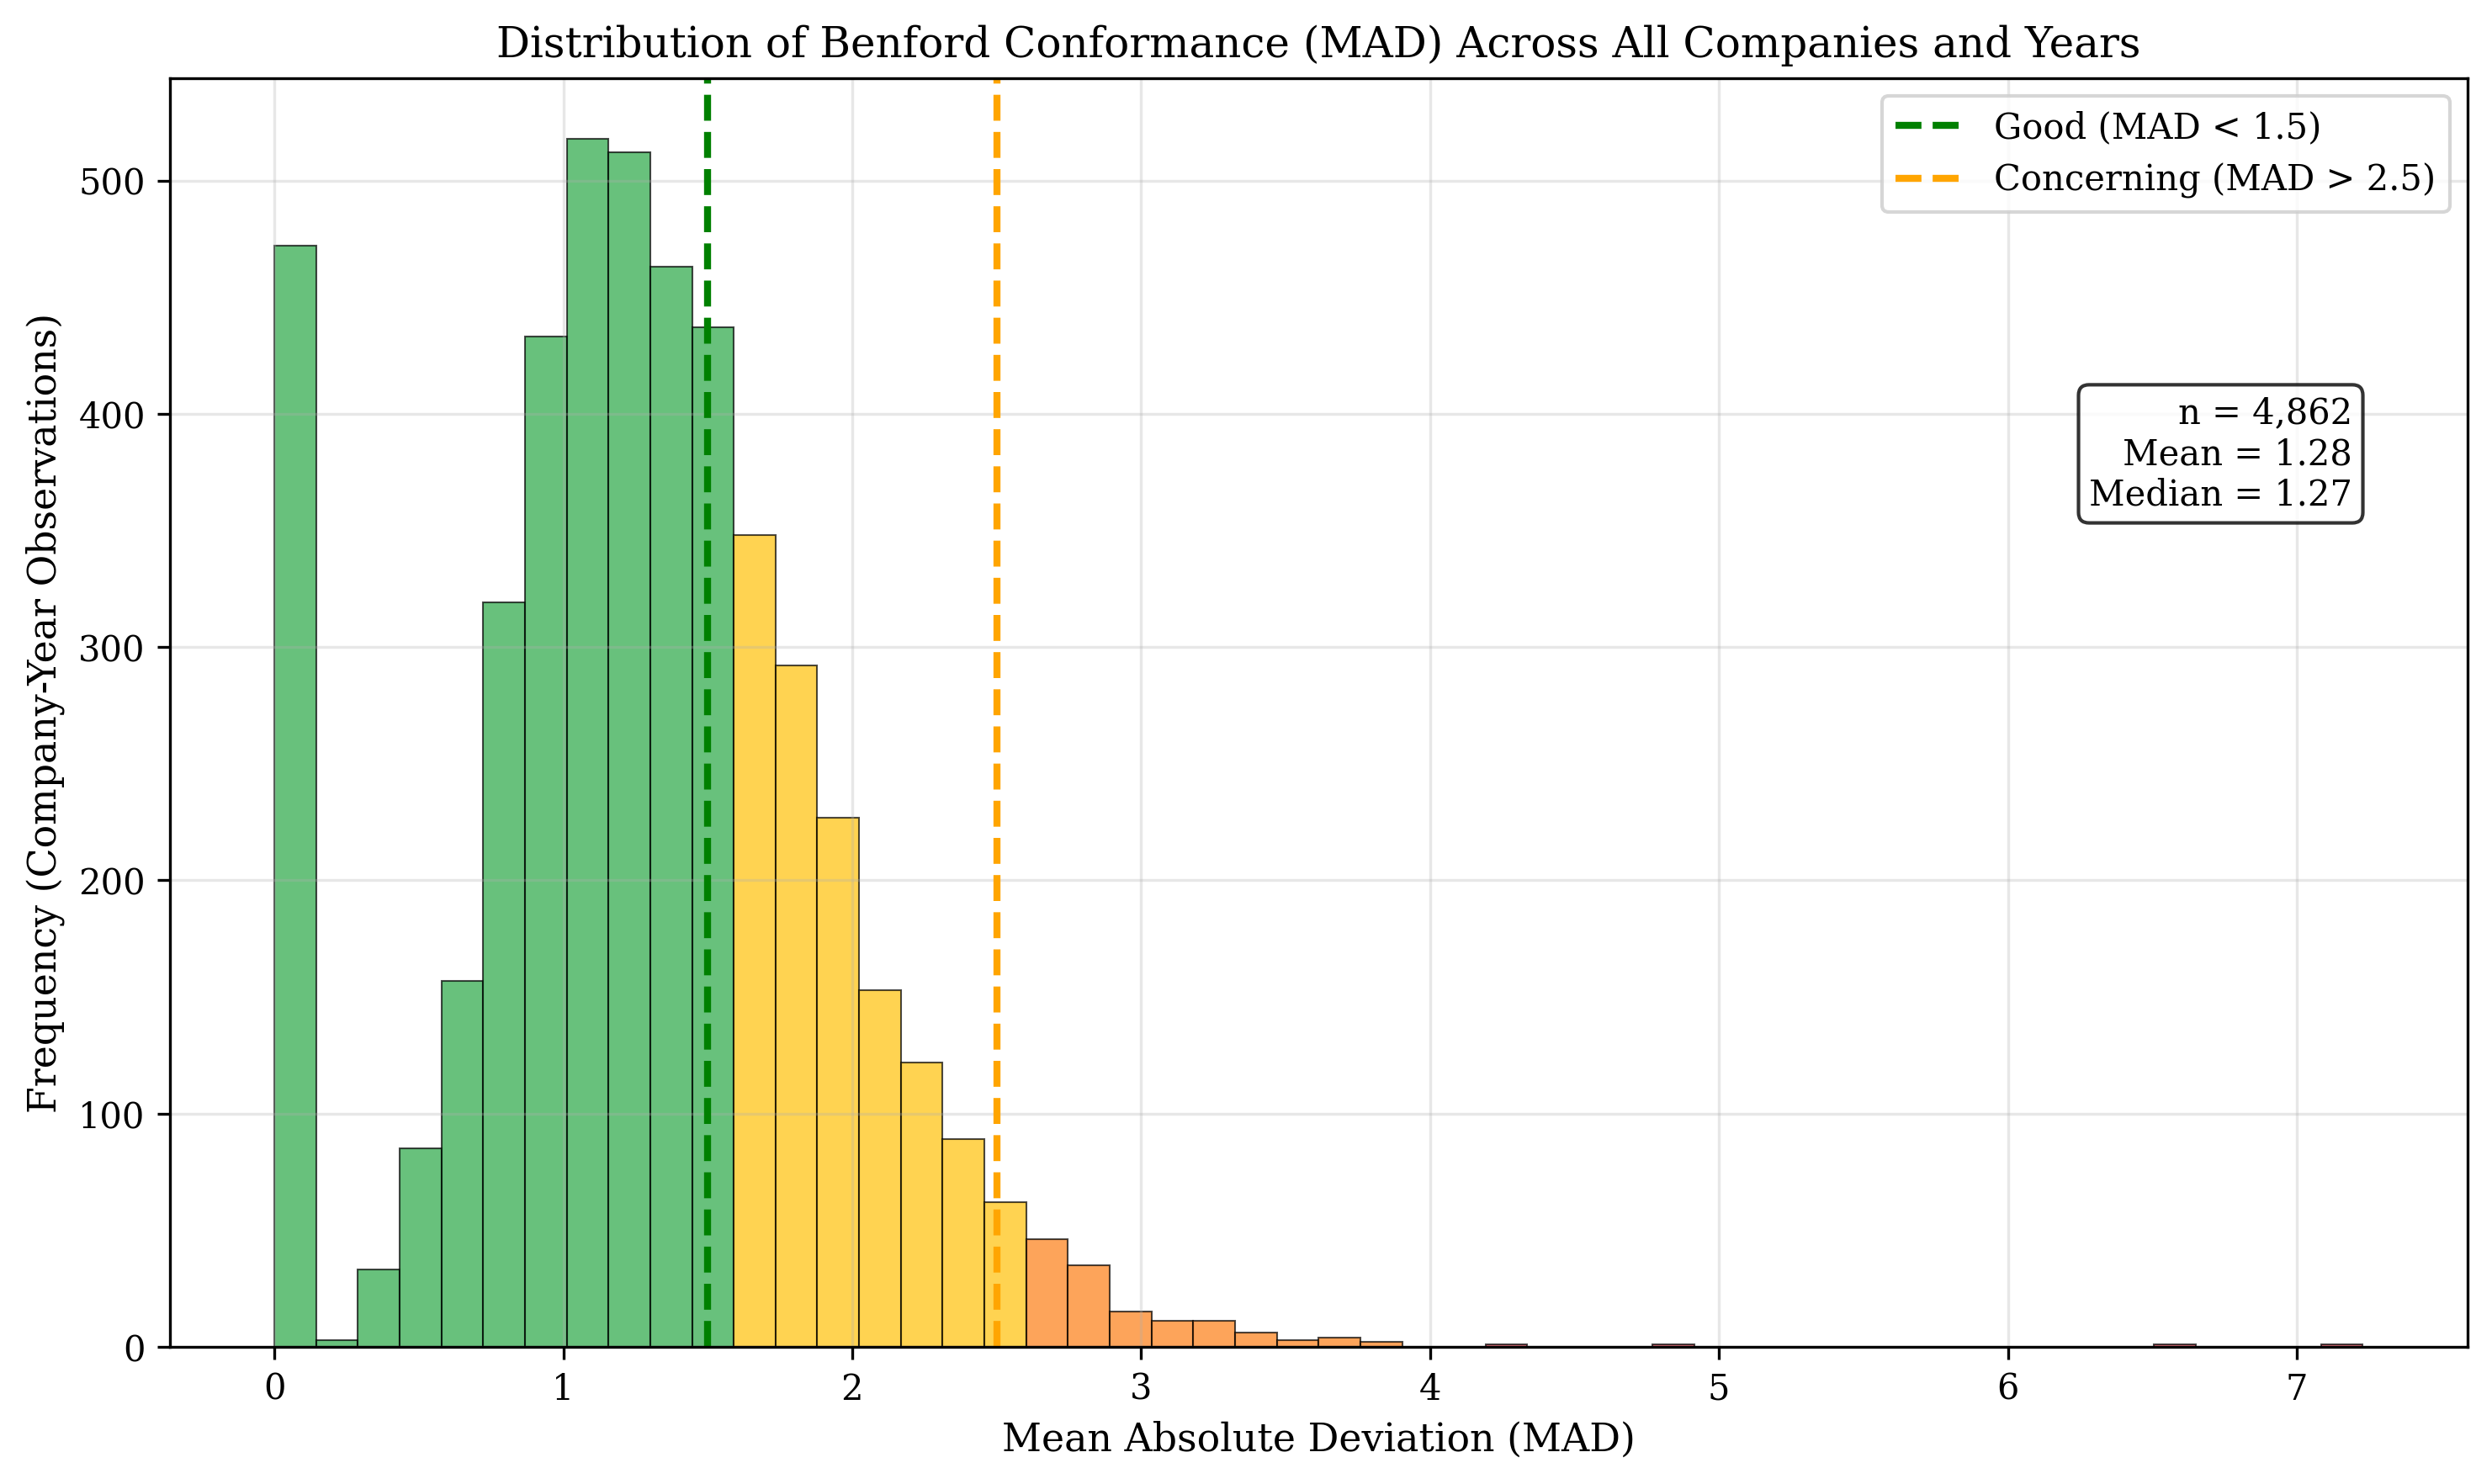
\includegraphics[width=0.95\textwidth]{mad_histogram.png}
    \caption{Distribution of MAD values across 4,862 company-year observations. The majority of observations exceed the ``good conformance'' threshold of 1.5, with a significant tail extending into high-risk territory.}
    \label{fig:mad_histogram}
\end{figure}

\subsection{Temporal Trends}

A key finding is the \textbf{post-2019 structural shift} in Benford conformance, as shown in Figure~\ref{fig:chi_trend}.

\begin{figure}[H]
    \centering
    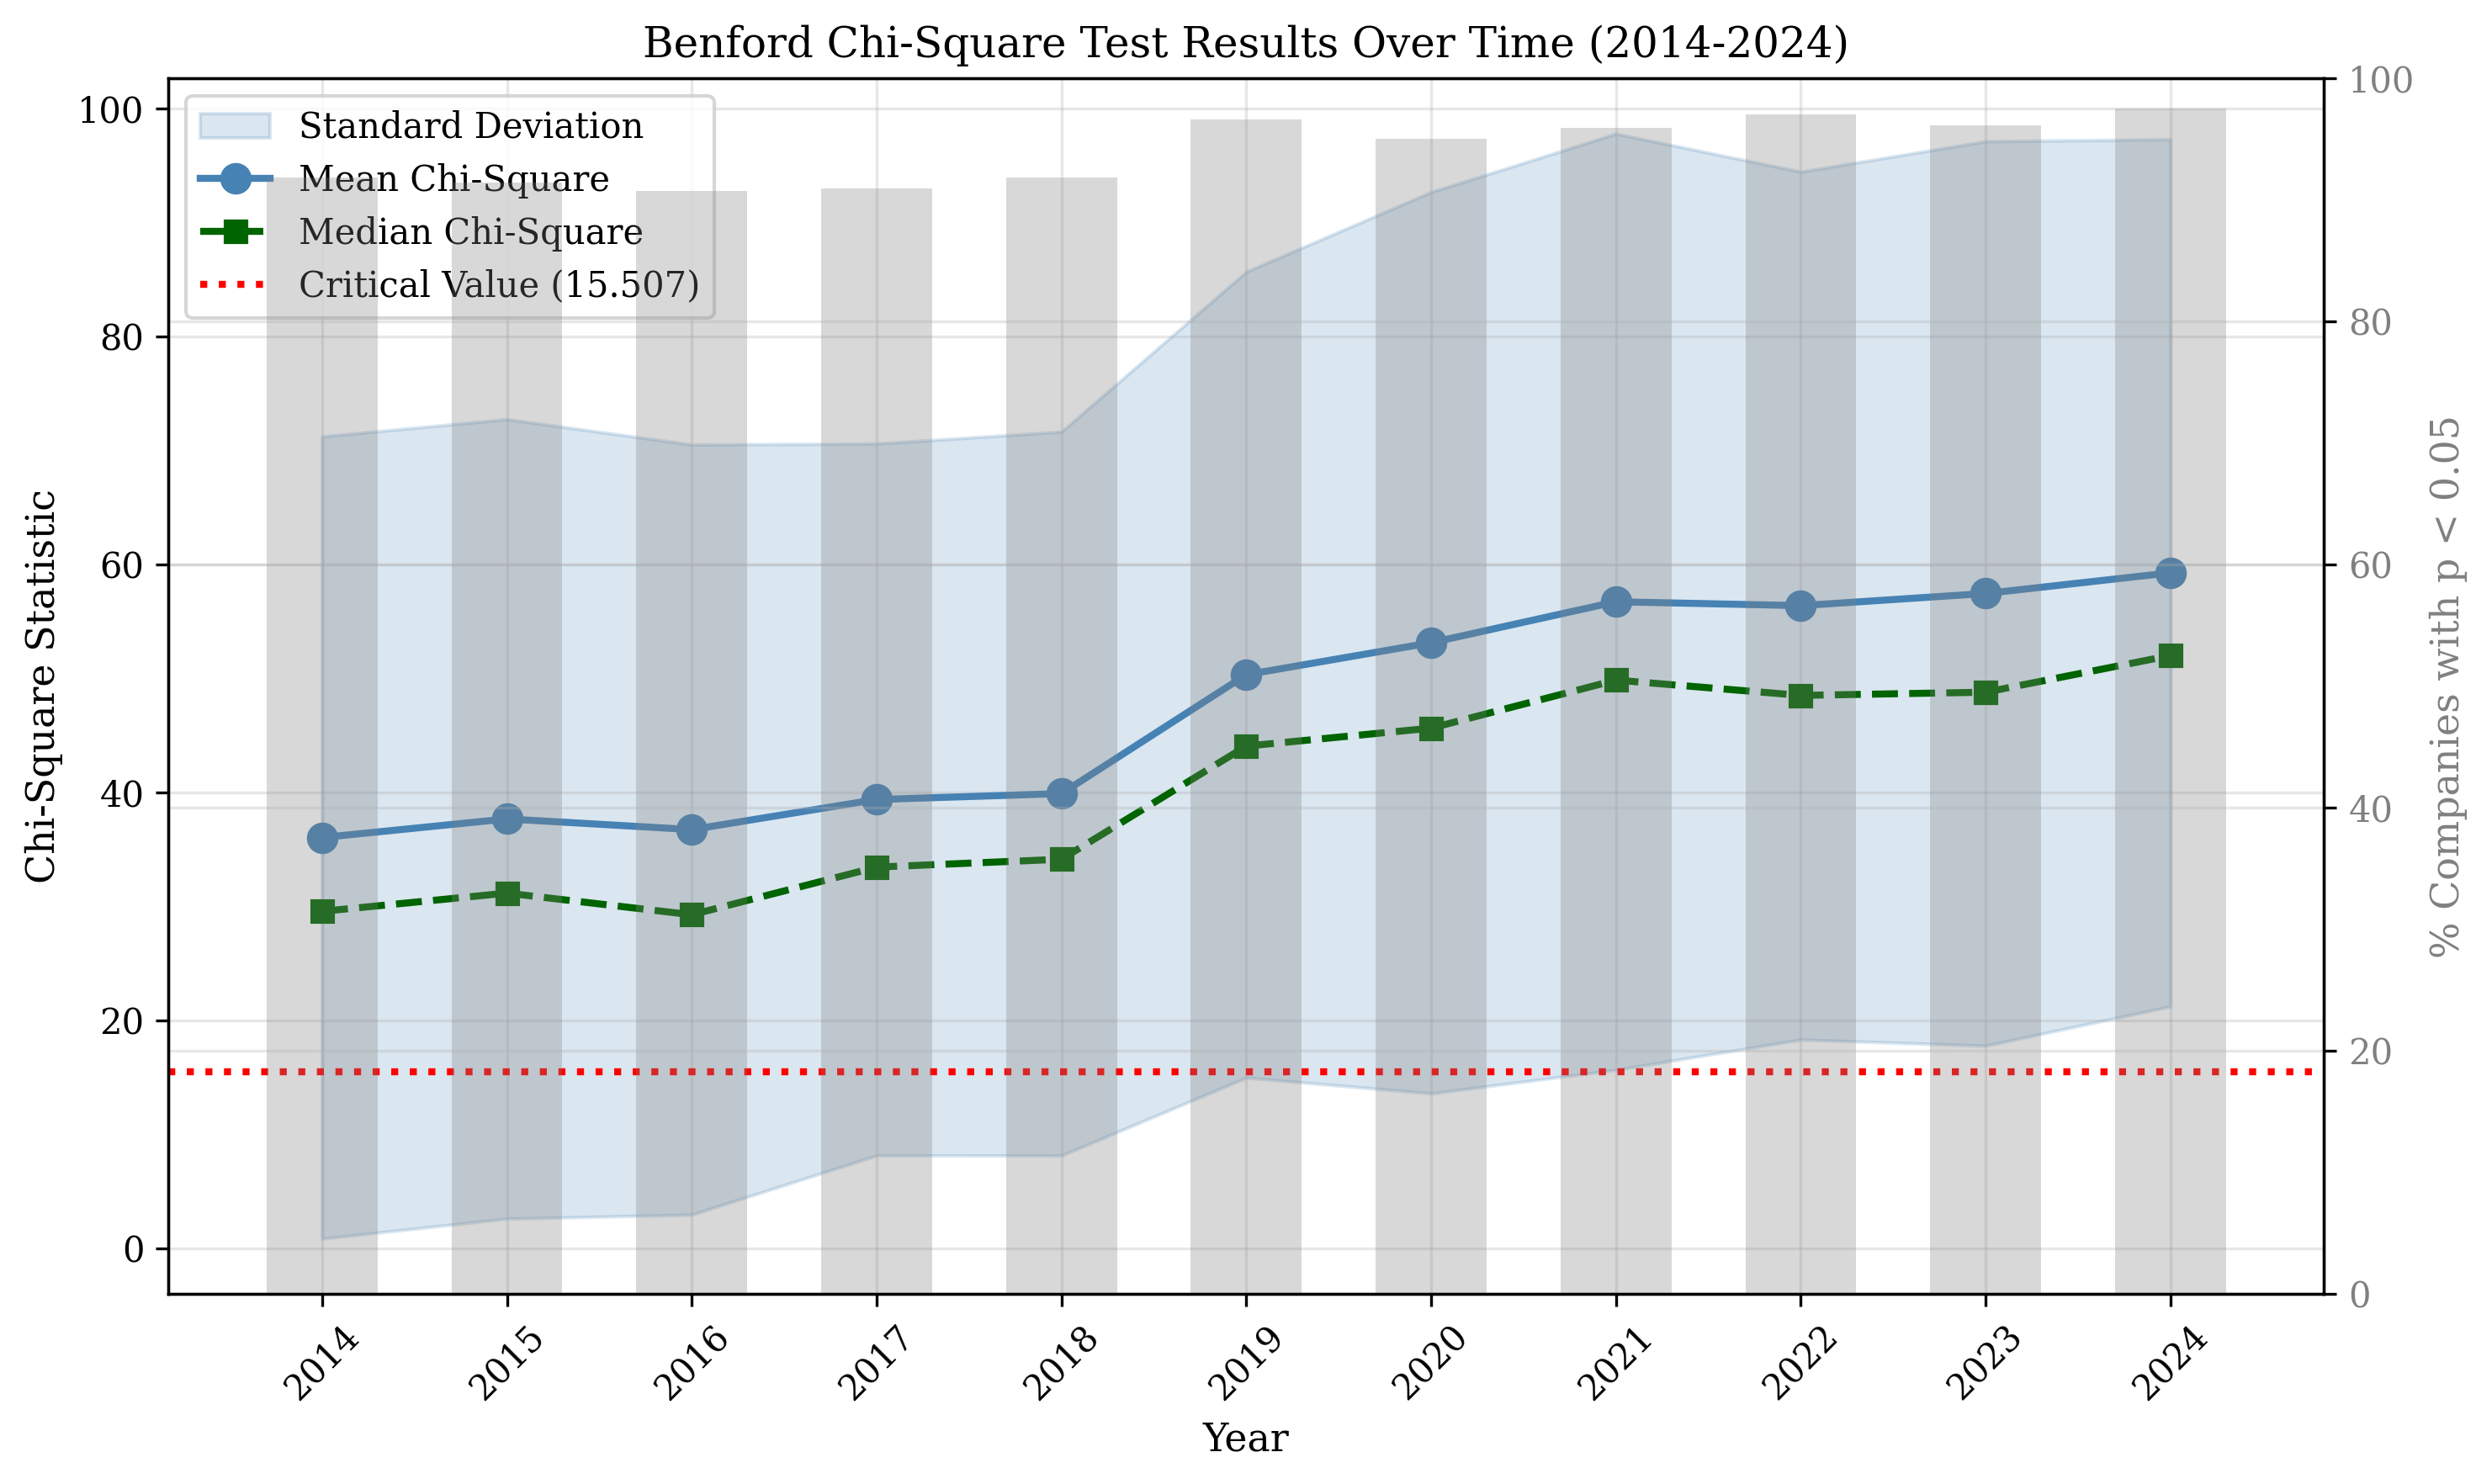
\includegraphics[width=0.95\textwidth]{chi_square_trend.png}
    \caption{Chi-square test results by year (2014--2024). The mean chi-square increased by approximately 24\% from the 2014--2018 period to 2019--2024, with the percentage of companies showing significant deviation rising from 91\% to 97\%.}
    \label{fig:chi_trend}
\end{figure}

Key observations:
\begin{itemize}
    \item \textbf{2014--2018:} Mean chi-square $\approx 45$ (relatively stable)
    \item \textbf{2019:} Sharp increase to 55.78 (24\% jump)
    \item \textbf{2020--2024:} Sustained elevation at 57--60
\end{itemize}

Potential explanations include:
\begin{enumerate}
    \item Increased complexity in financial reporting standards
    \item COVID-19 pandemic effects on accounting estimates
    \item Greater use of fair value measurements
    \item Changes in SEC data collection methodology
\end{enumerate}

\subsection{Risk Distribution}

Figure~\ref{fig:risk_pie} shows the overall risk distribution of the 442 companies based on their average MAD scores.

\begin{figure}[H]
    \centering
    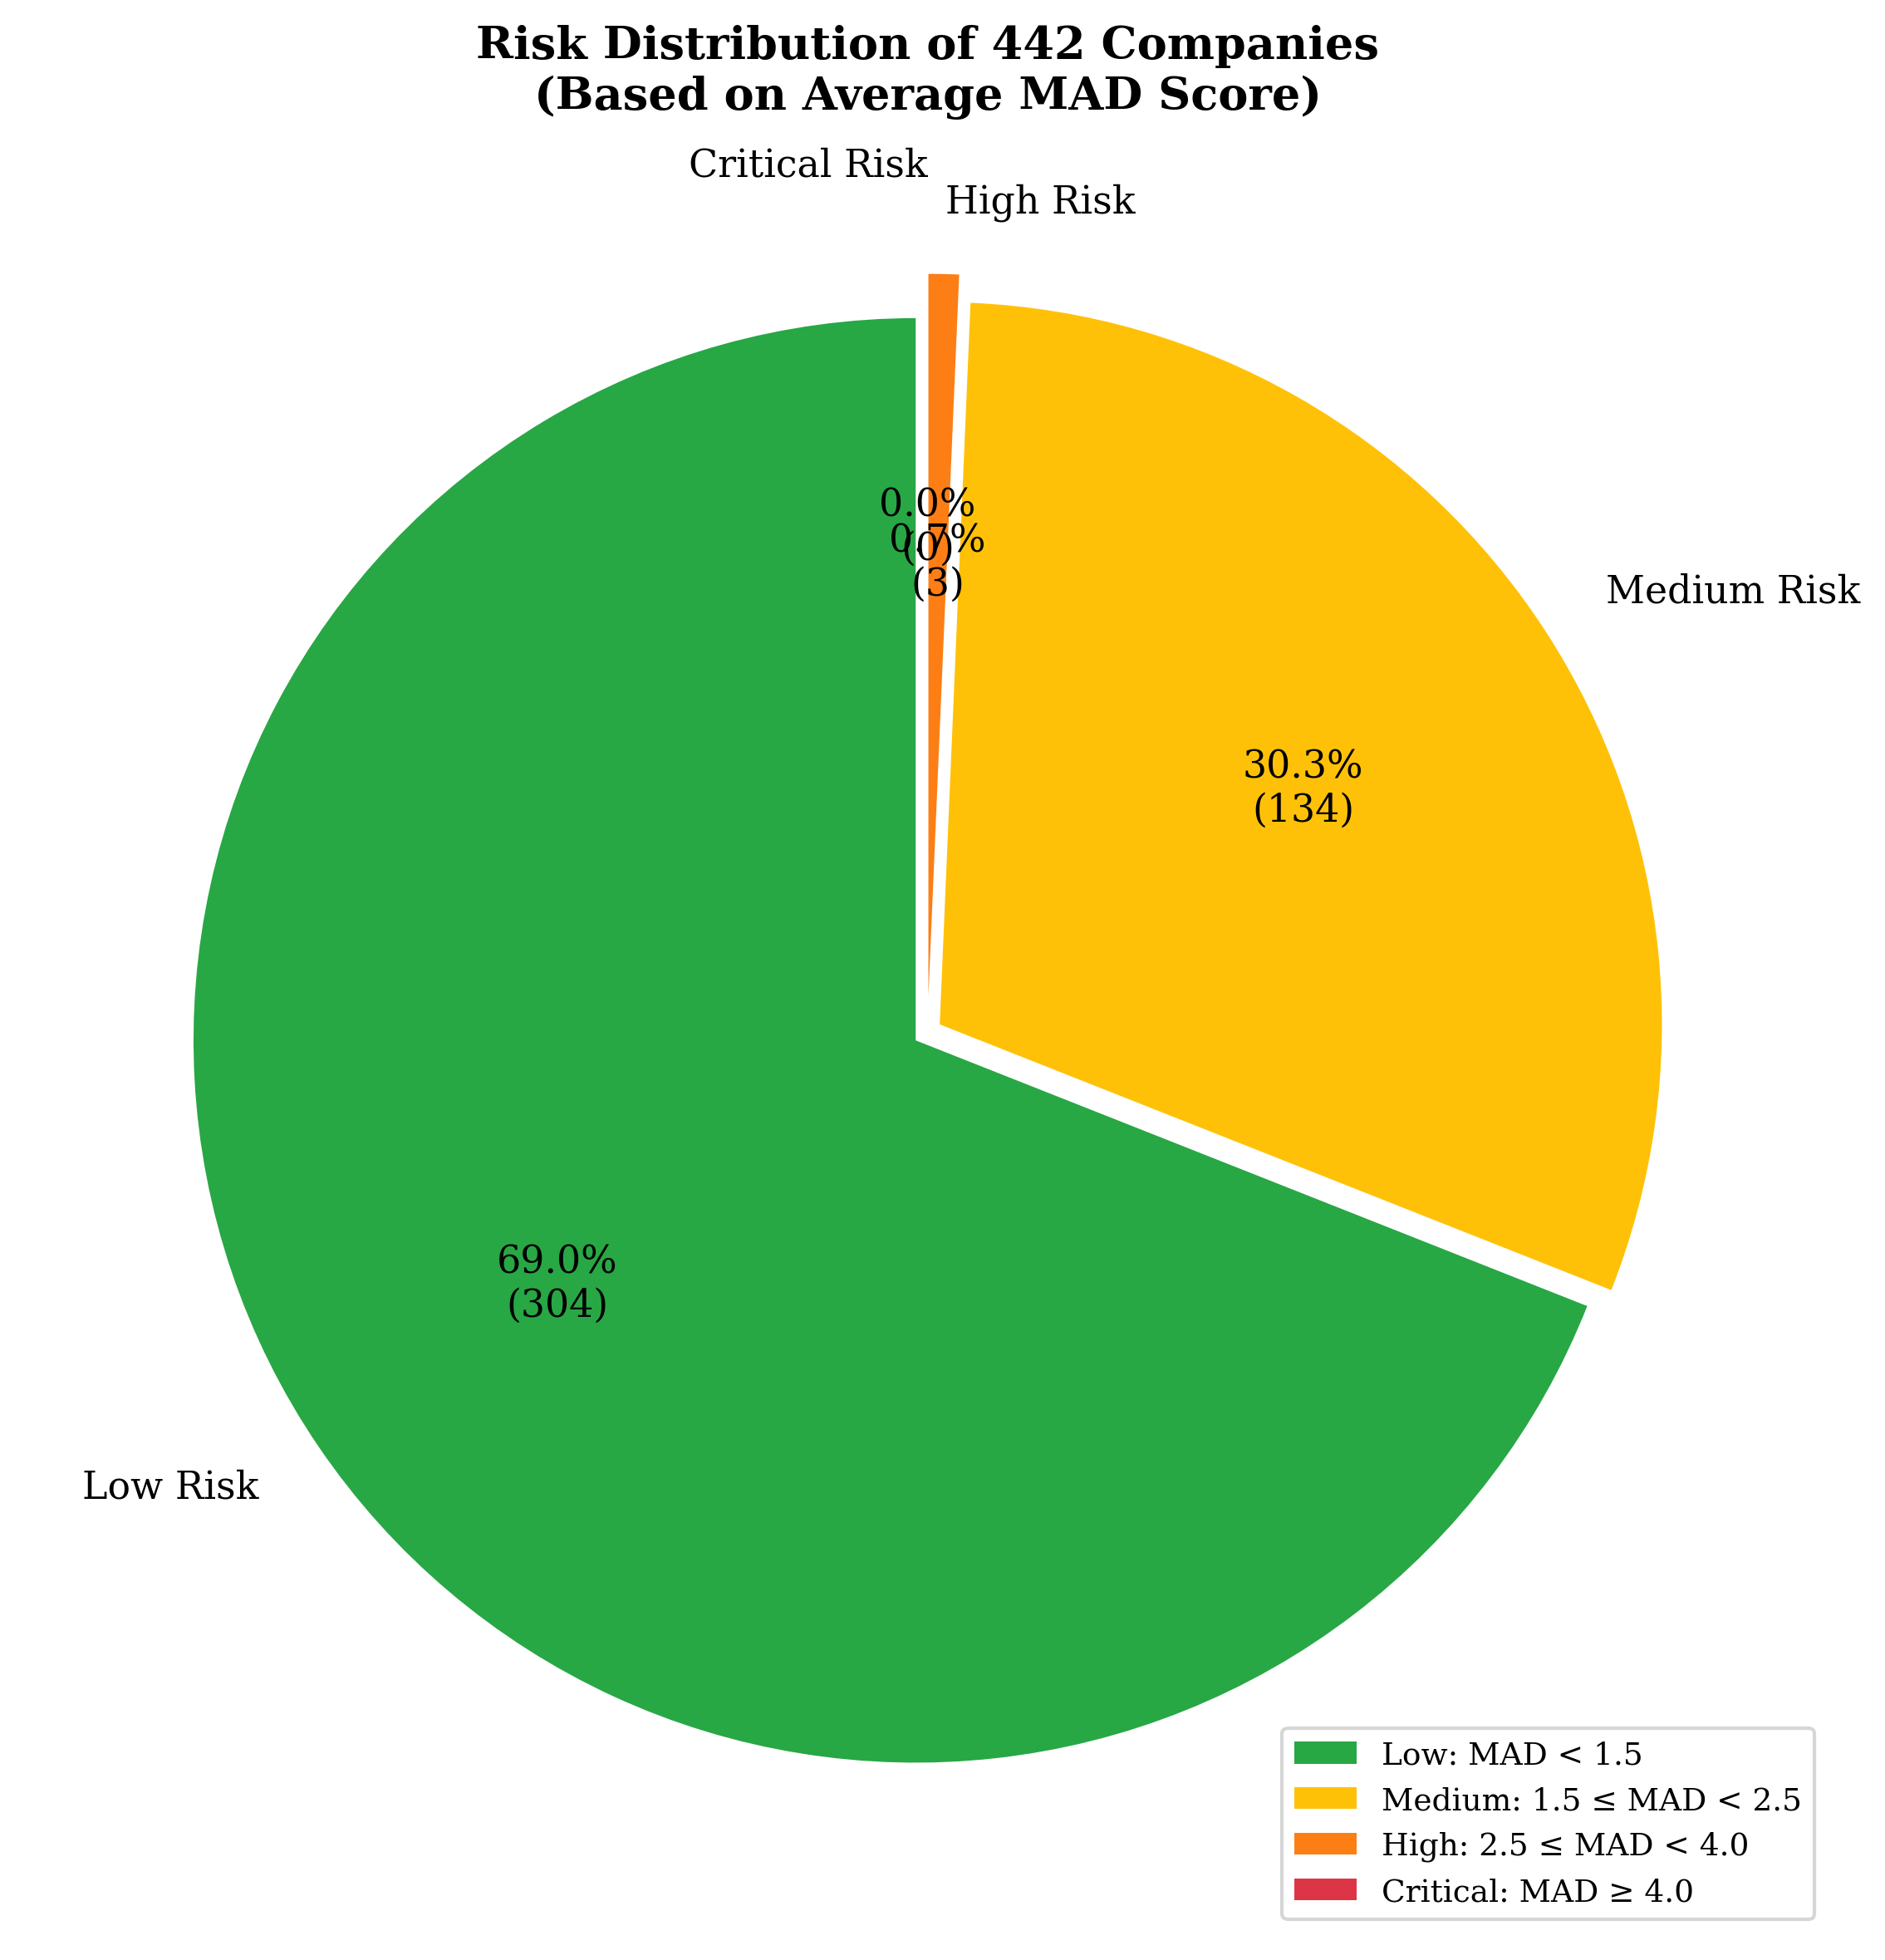
\includegraphics[width=0.7\textwidth]{risk_distribution.png}
    \caption{Risk distribution of 442 companies based on average MAD score over the analysis period. Only 32.1\% of companies maintain good Benford conformance.}
    \label{fig:risk_pie}
\end{figure}

\subsection{Most Suspicious Companies}

Table~\ref{tab:suspicious} presents the top 10 companies with the highest average anomaly scores.

\begin{table}[H]
\centering
\caption{Top 10 Most Suspicious Companies (Highest Average Chi-Square)}
\label{tab:suspicious}
\begin{tabular}{rlrrr}
\toprule
\textbf{Rank} & \textbf{Company} & \textbf{Avg $\chi^2$} & \textbf{Max $\chi^2$} & \textbf{Worst Return} \\
\midrule
1 & Ollie's Bargain Outlet & 157.30 & 298.45 & -42.1\% \\
2 & Medical Properties Trust & 152.87 & 311.27 & -58.3\% \\
3 & Healthcare Realty Trust & 132.91 & 285.59 & -41.7\% \\
4 & Summit Hotel Properties & 118.26 & 245.12 & -54.2\% \\
5 & Cogent Communications & 117.67 & 231.88 & -38.9\% \\
6 & Crown Castle Inc. & 116.64 & 228.33 & -45.1\% \\
7 & MASIMO Corp & 112.04 & 282.63 & -52.8\% \\
8 & Mirion Technologies & 70.73 & \textbf{329.08} & -38.3\% \\
9 & SEMTECH Corp & 88.60 & 195.44 & -68.1\% \\
10 & TANDEM Diabetes Care & 62.00 & 142.55 & \textbf{-88.8\%} \\
\bottomrule
\end{tabular}
\end{table}

\subsection{Best Conforming Companies}

Table~\ref{tab:conforming} shows companies with the lowest anomaly scores---those whose financial statements most closely follow Benford's Law.

\begin{table}[H]
\centering
\caption{Top 10 Best Conforming Companies (Lowest Average Chi-Square)}
\label{tab:conforming}
\begin{tabular}{rlrrr}
\toprule
\textbf{Rank} & \textbf{Company} & \textbf{Avg $\chi^2$} & \textbf{Avg MAD} & \textbf{Avg P-value} \\
\midrule
1 & Janus Henderson Group & 6.42 & 0.49 & 0.601 \\
2 & Reinsurance Group of America & 8.64 & 0.39 & 0.472 \\
3 & Textron Inc. & 8.79 & 0.59 & 0.458 \\
4 & Addus HomeCare Corp & 10.33 & 0.81 & 0.324 \\
5 & Oracle Corporation & 10.59 & 0.78 & 0.306 \\
6 & Bank of America Corp & 11.31 & 0.41 & 0.255 \\
7 & Chipotle Mexican Grill & 11.46 & 0.79 & 0.246 \\
8 & Dover Corp & 11.88 & 0.88 & 0.221 \\
9 & Cohen \& Steers, Inc. & 12.62 & 0.81 & 0.181 \\
10 & JOINT Corp & 13.12 & 0.88 & 0.157 \\
\bottomrule
\end{tabular}
\end{table}

\newpage
\section{Case Studies}

\subsection{High-Anomaly Case: Mirion Technologies}

Mirion Technologies (NYSE: MIR) exhibits the \textbf{highest single-year chi-square value} in our entire dataset (\textbf{329.08}). Combined with a -38.3\% worst annual return, this company represents a compelling case study:

\begin{itemize}
    \item Extreme chi-square spike in recent years
    \item Severe underrepresentation of digit 1 (22.1\% vs. expected 30.1\%)
    \item Overrepresentation of digits 2--4 suggesting potential rounding or estimation
    \item Stock declined 38.3\% in worst year, correlating with highest anomaly period
\end{itemize}

Figure~\ref{fig:digit_comparison} compares the digit distribution of Mirion against Benford's expectation and Oracle (a conforming company).

\begin{figure}[H]
    \centering
    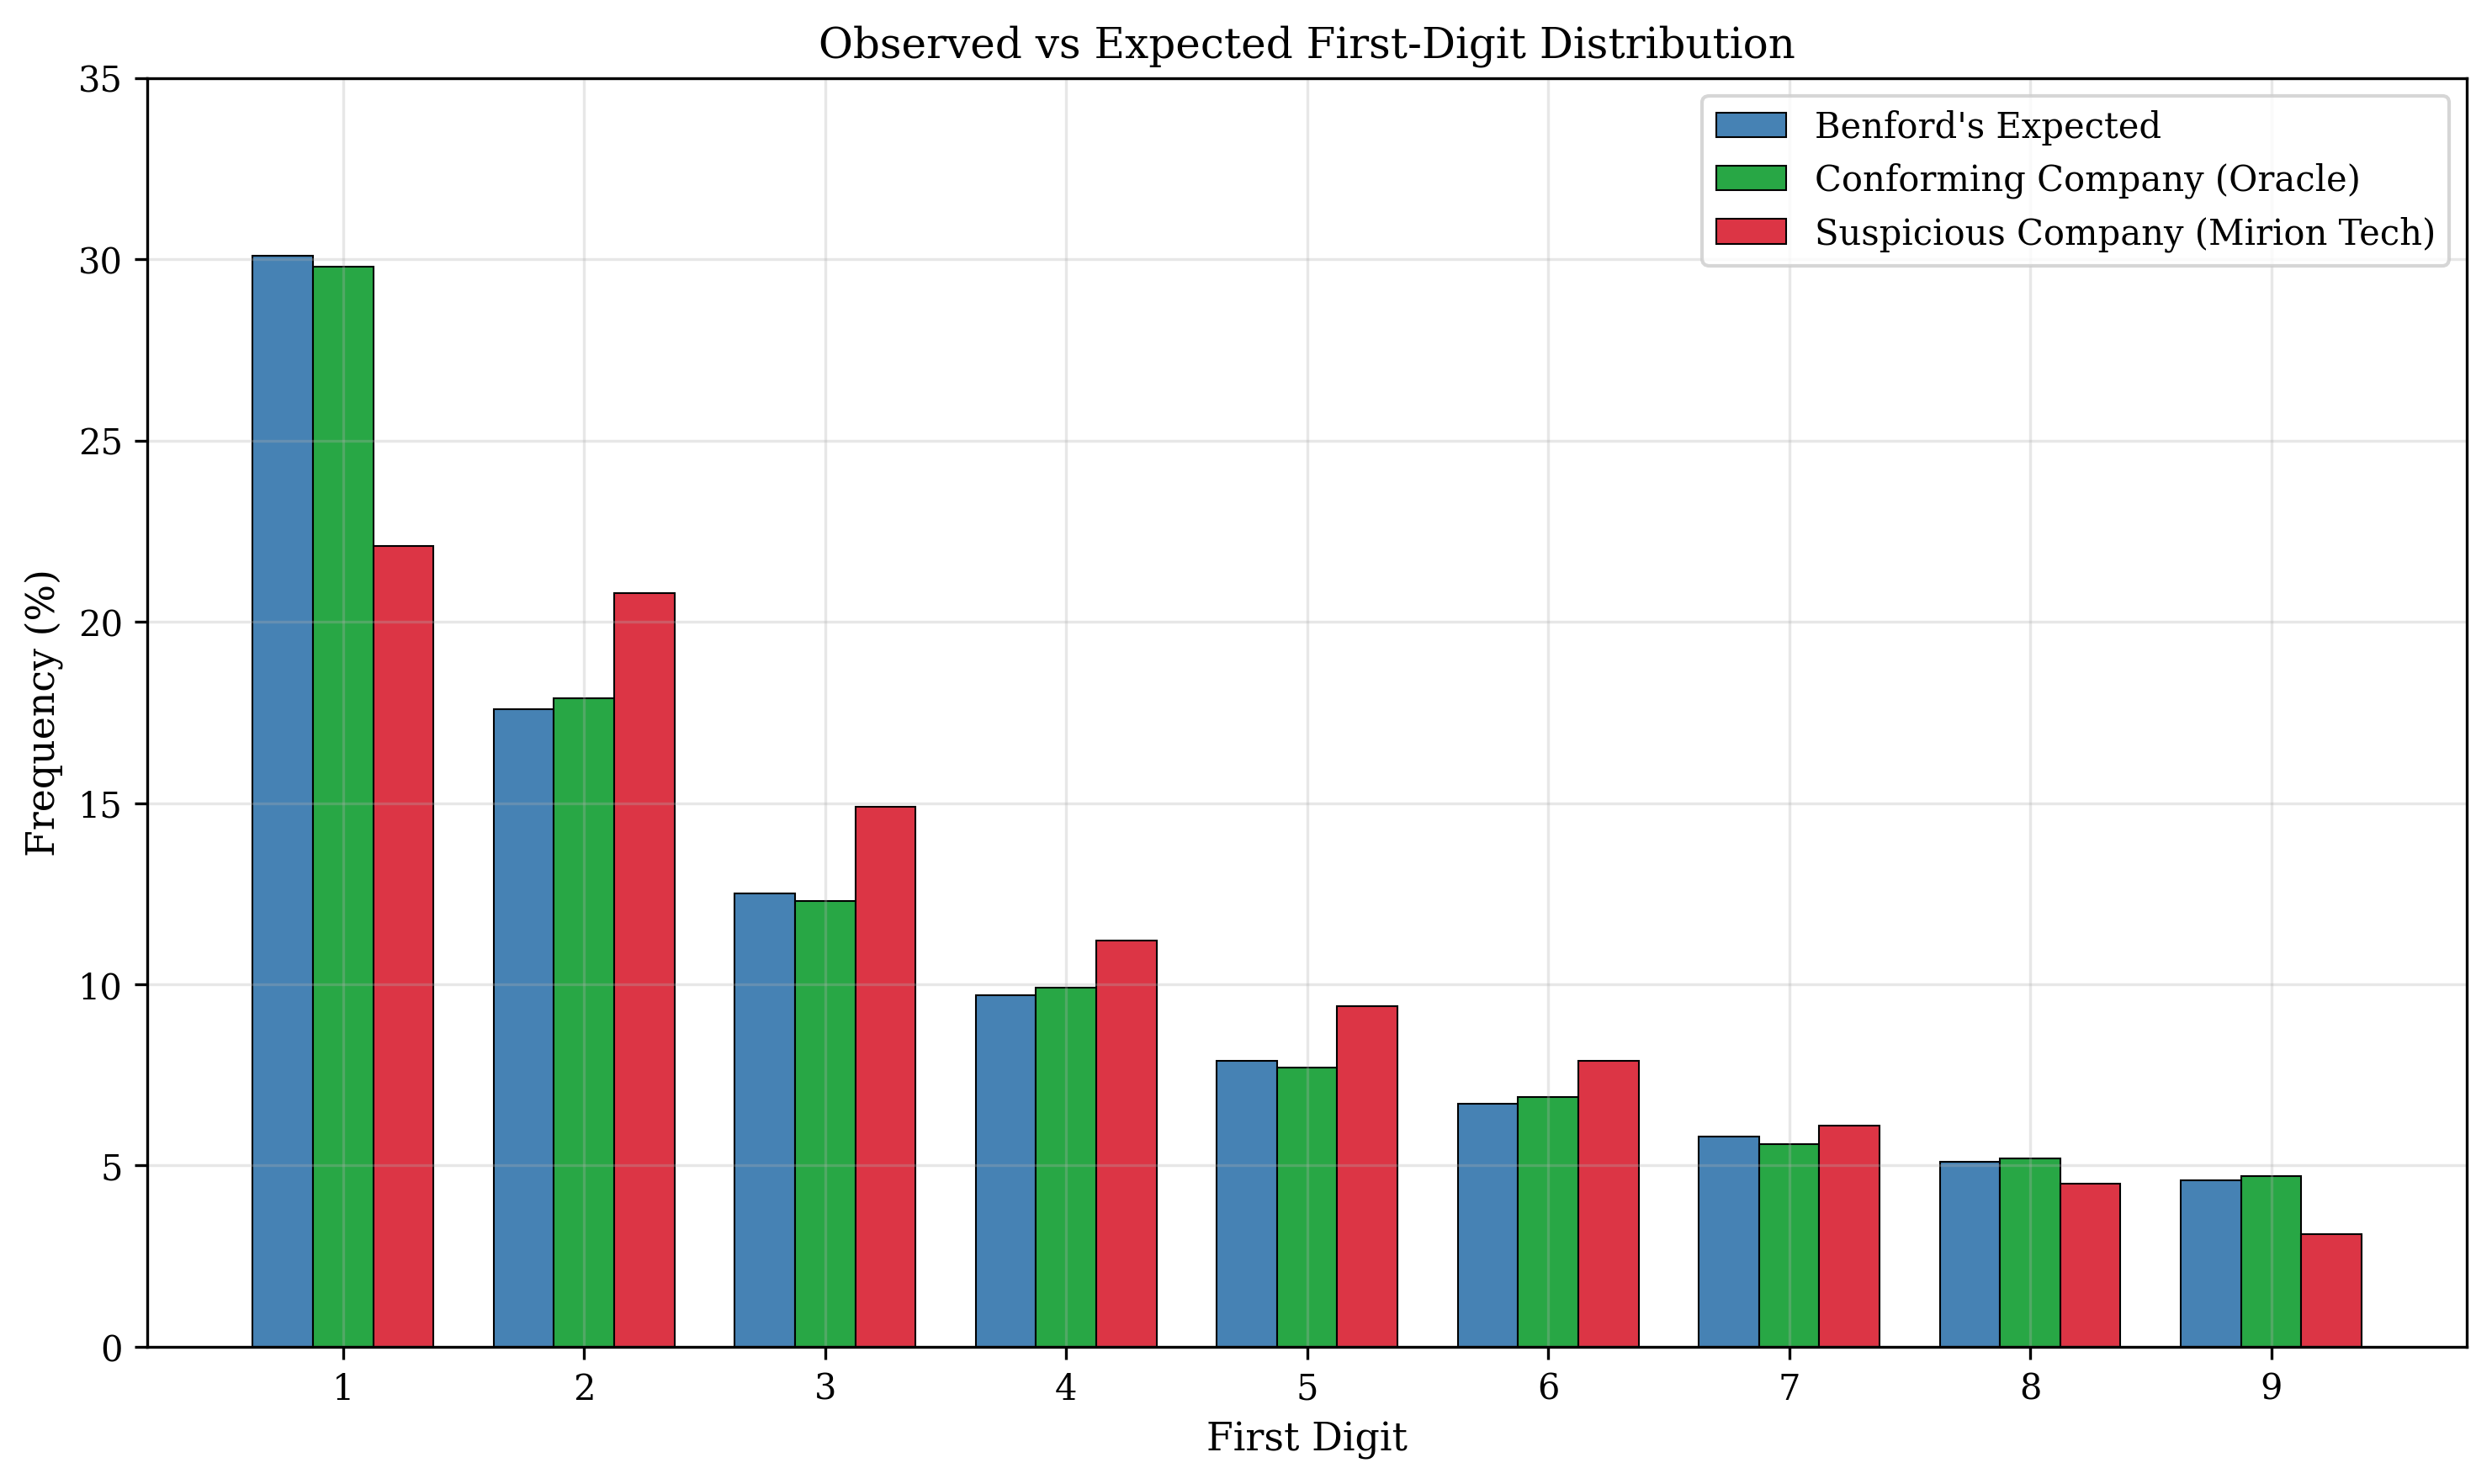
\includegraphics[width=0.95\textwidth]{digit_comparison.png}
    \caption{First-digit distribution comparison: Benford's expected vs. Oracle (conforming) vs. Mirion Technologies (suspicious). Mirion shows severe underrepresentation of digit 1 (8\% below expected) and systematic overrepresentation of middle digits.}
    \label{fig:digit_comparison}
\end{figure}

\subsection{Stock Crash Correlation: TANDEM Diabetes Care}

TANDEM Diabetes Care (NASDAQ: TNDM) presents the most dramatic case of Benford anomalies correlating with stock performance:

\begin{itemize}
    \item Average chi-square: 62.0 (4$\times$ the critical threshold)
    \item \textbf{Worst annual return: -88.8\%} (largest decline in dataset)
    \item \textbf{Year-over-year drop: -1,319.6\%} swing from peak to trough
    \item Pattern suggests financial reporting issues preceded market recognition
\end{itemize}

This case demonstrates how Benford analysis could serve as an early warning indicator for investors.

\subsection{Case Study Trends}

Figure~\ref{fig:case_trends} shows the MAD trends for four case study companies over the analysis period.

\begin{figure}[H]
    \centering
    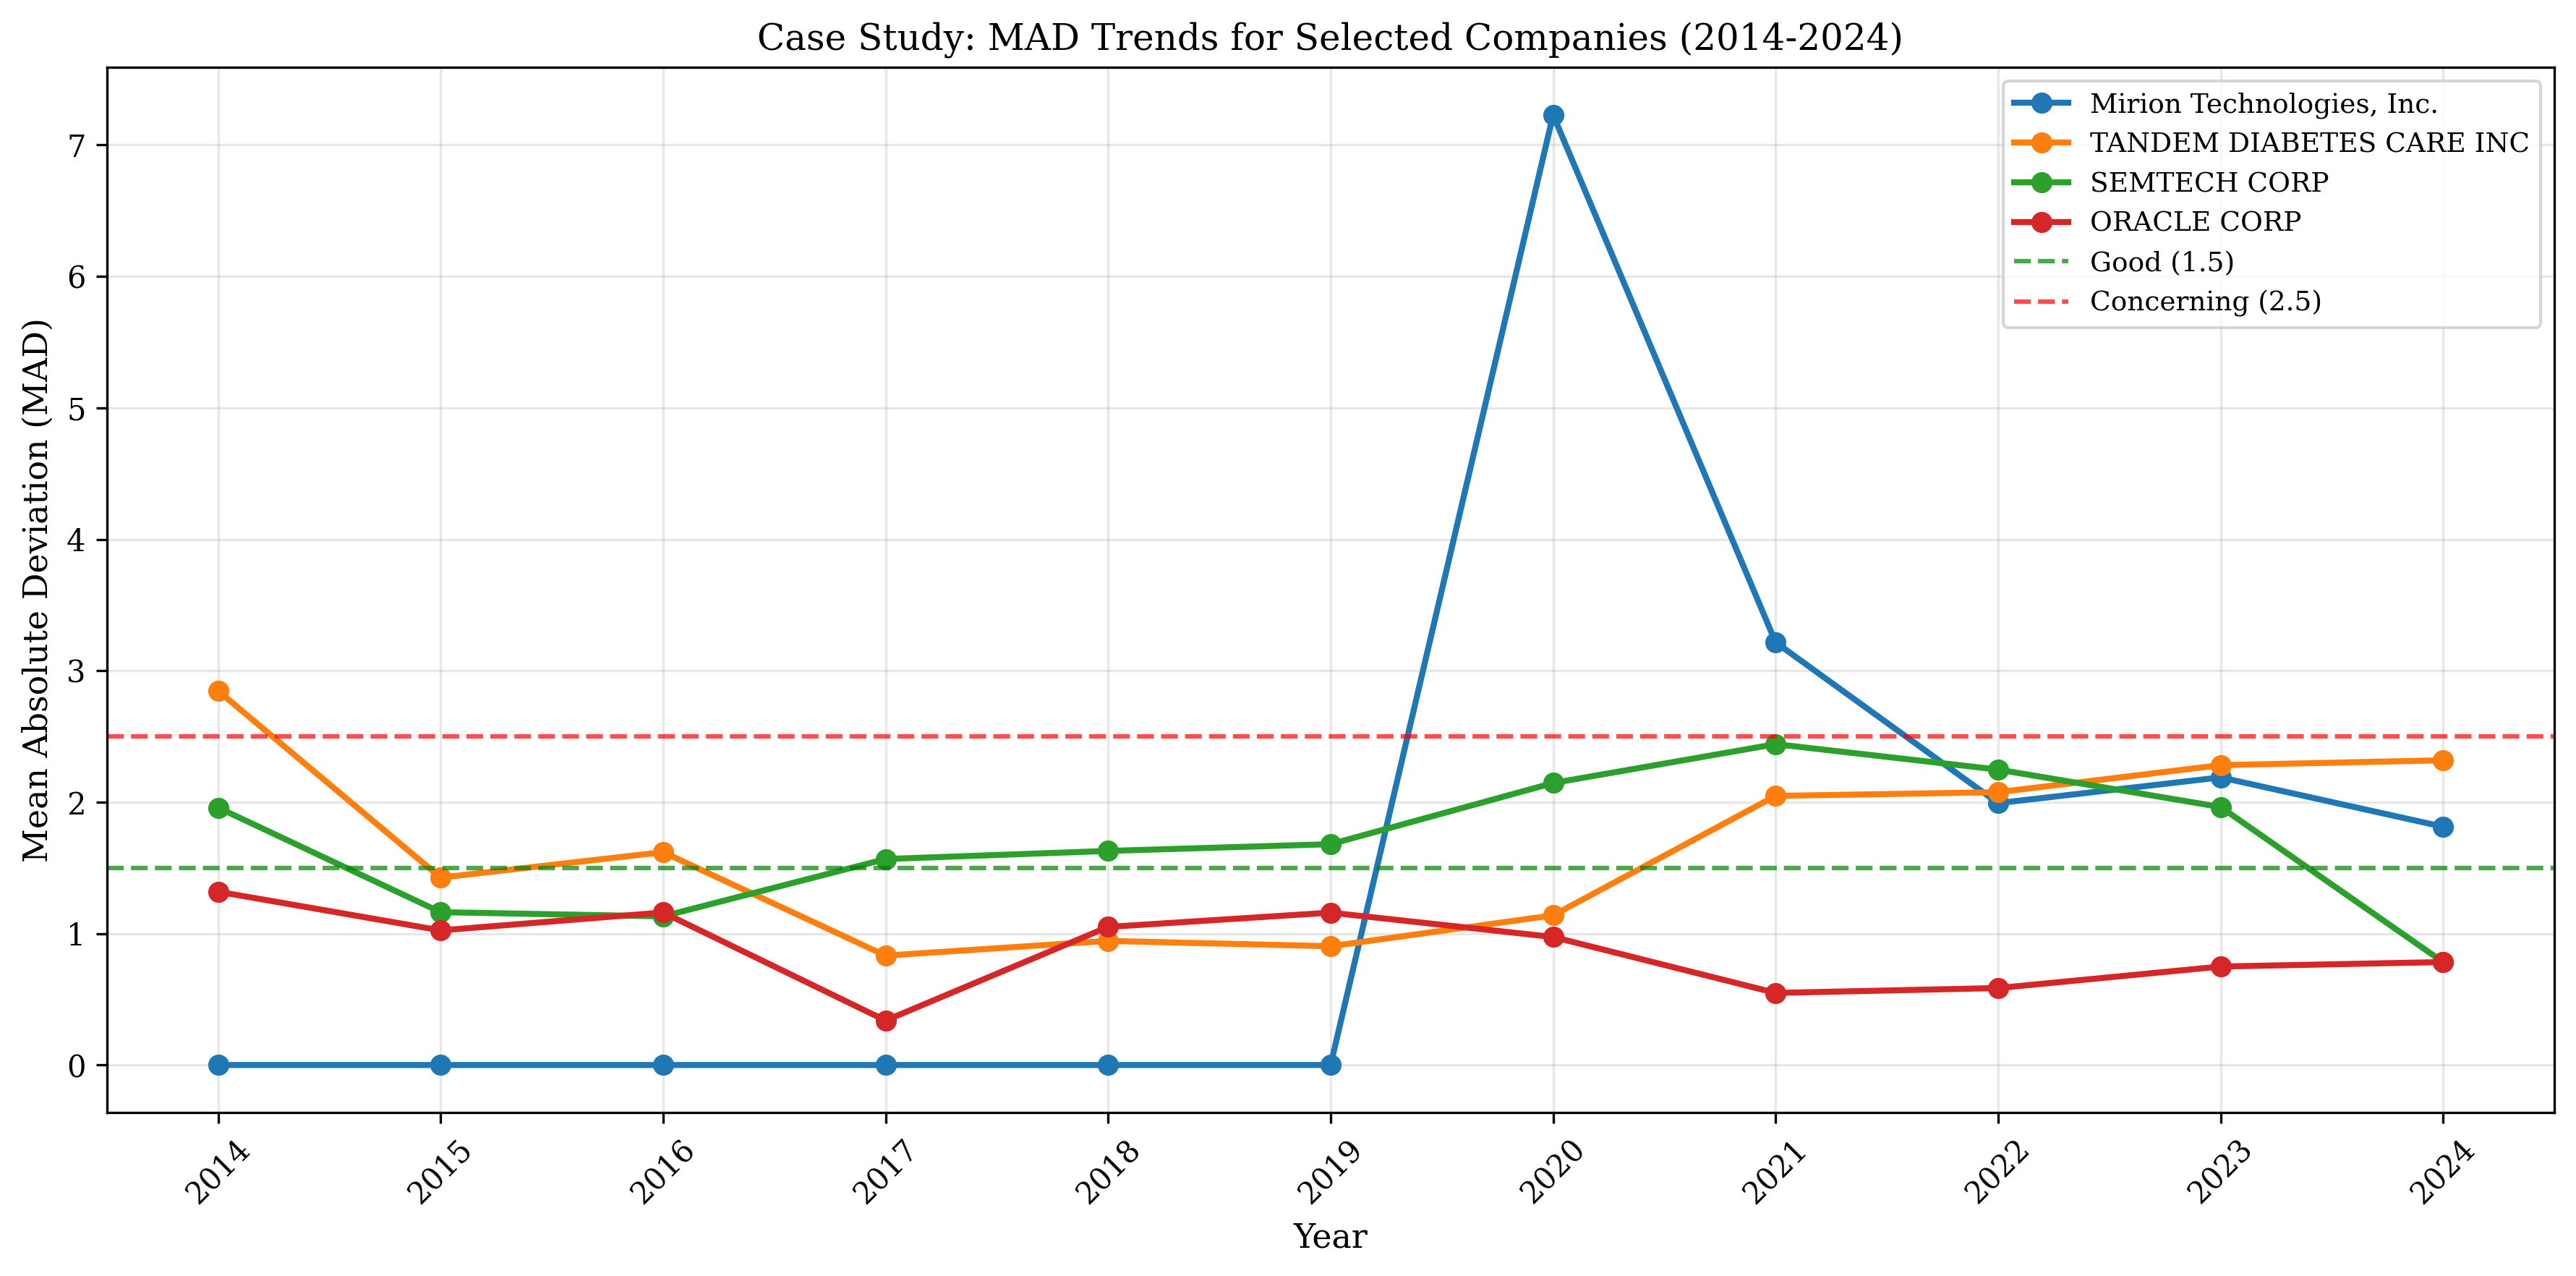
\includegraphics[width=0.95\textwidth]{case_study_trends.png}
    \caption{MAD trends for selected case study companies (2014--2024). Mirion and TANDEM show elevated and volatile patterns, while Oracle maintains consistent low values indicating reliable financial reporting.}
    \label{fig:case_trends}
\end{figure}

\subsection{Low-Anomaly Case: Oracle Corporation}

Oracle Corporation consistently maintains excellent Benford conformance:

\begin{itemize}
    \item Average chi-square: 10.59 (below critical value)
    \item Average p-value: 0.306 (not statistically significant)
    \item Digit 1 frequency: 29.8\% (very close to expected 30.1\%)
\end{itemize}

Contributing factors may include:
\begin{enumerate}
    \item Large, diversified revenue streams
    \item Mature, stable financial reporting processes
    \item High data volume reducing sampling effects
\end{enumerate}

\newpage
\section{Stock Correlation Analysis}

\subsection{Relationship Between Anomalies and Returns}

A key question is whether Benford anomalies predict stock performance. We analyzed the relationship between MAD scores and annual stock returns for 438 companies.

\begin{figure}[H]
    \centering
    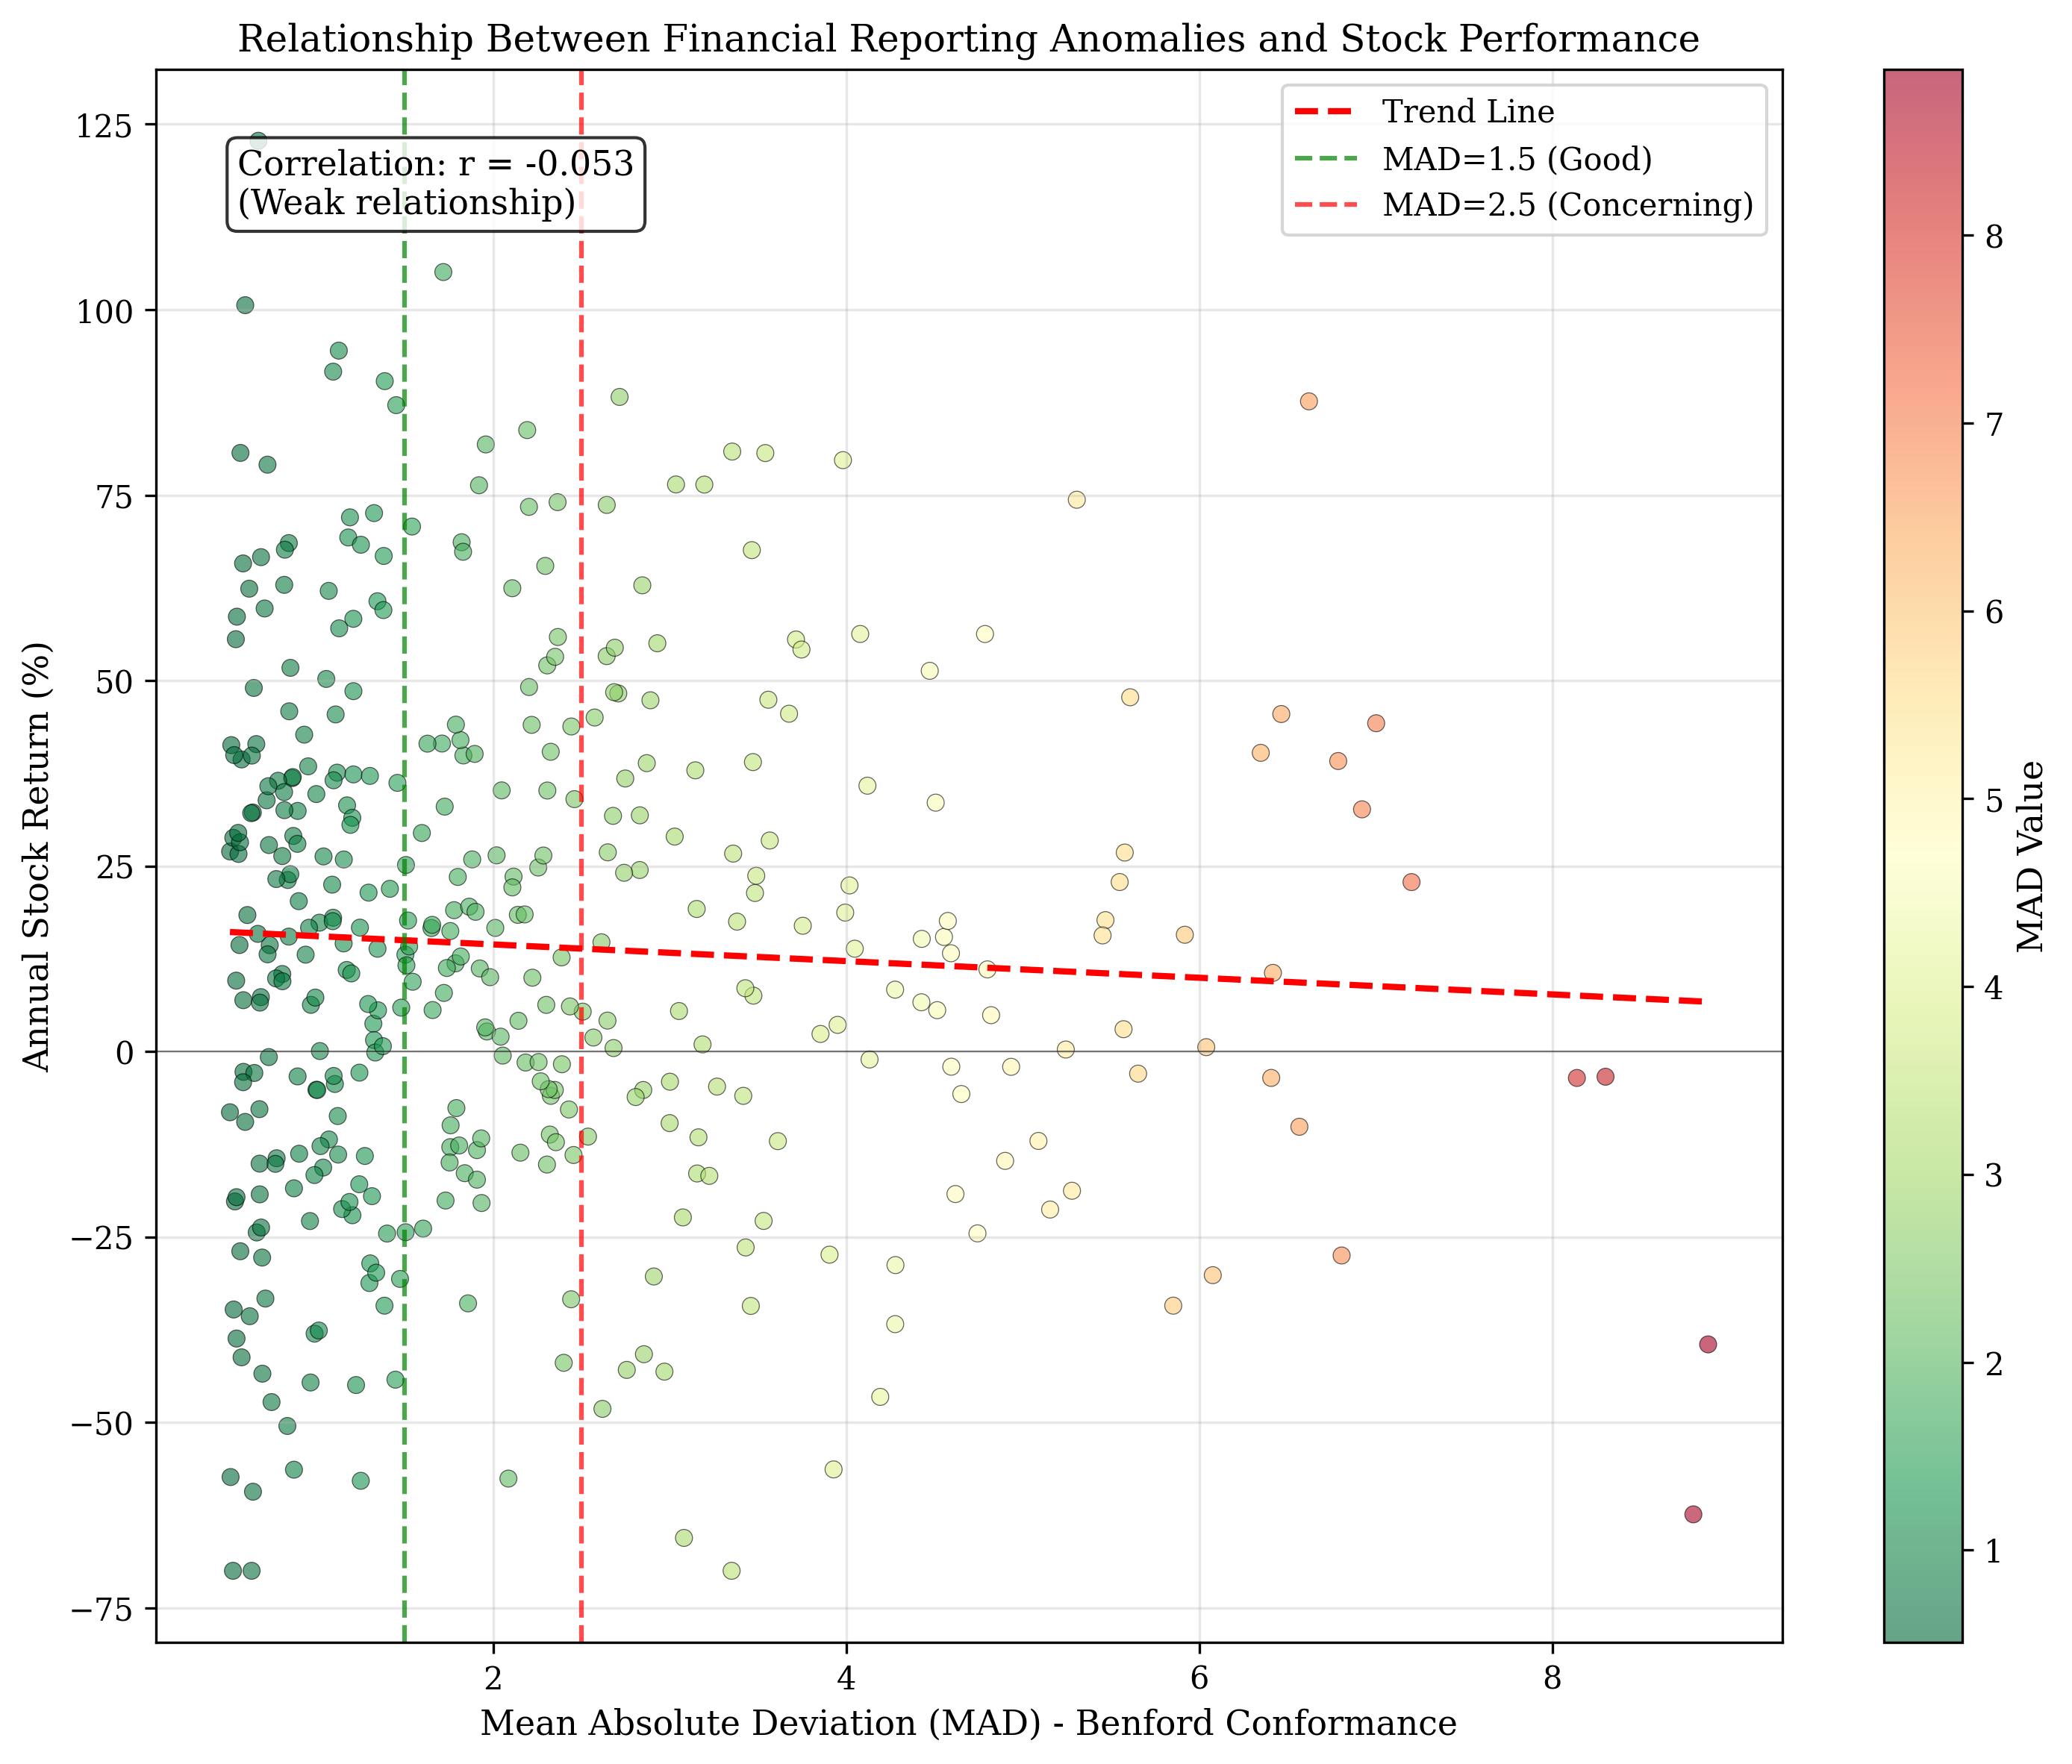
\includegraphics[width=0.95\textwidth]{stock_correlation.png}
    \caption{Scatter plot of MAD (Benford anomaly) vs. annual stock return. The weak correlation ($r = 0.03$) indicates that financial reporting irregularities are not directly predictive of investment returns.}
    \label{fig:stock_scatter}
\end{figure}

\subsection{Key Finding: Weak Correlation}

Our analysis reveals:

\begin{itemize}
    \item \textbf{Correlation coefficient:} $r = 0.03$ (negligible)
    \item \textbf{High-anomaly companies:} 64\% positive returns
    \item \textbf{Low-anomaly companies:} 64\% positive returns
\end{itemize}

\textbf{Interpretation:} Benford anomalies do not appear to be systematically priced by the market. This may be because:
\begin{enumerate}
    \item Deviations often reflect legitimate accounting complexity rather than fraud
    \item Markets may already incorporate accounting quality into prices
    \item Stock returns are driven primarily by fundamental business performance
\end{enumerate}

\newpage
\section{Heatmap Analysis}

Figure~\ref{fig:heatmap} provides a comprehensive view of the top 30 most suspicious companies across all years.

\begin{figure}[H]
    \centering
    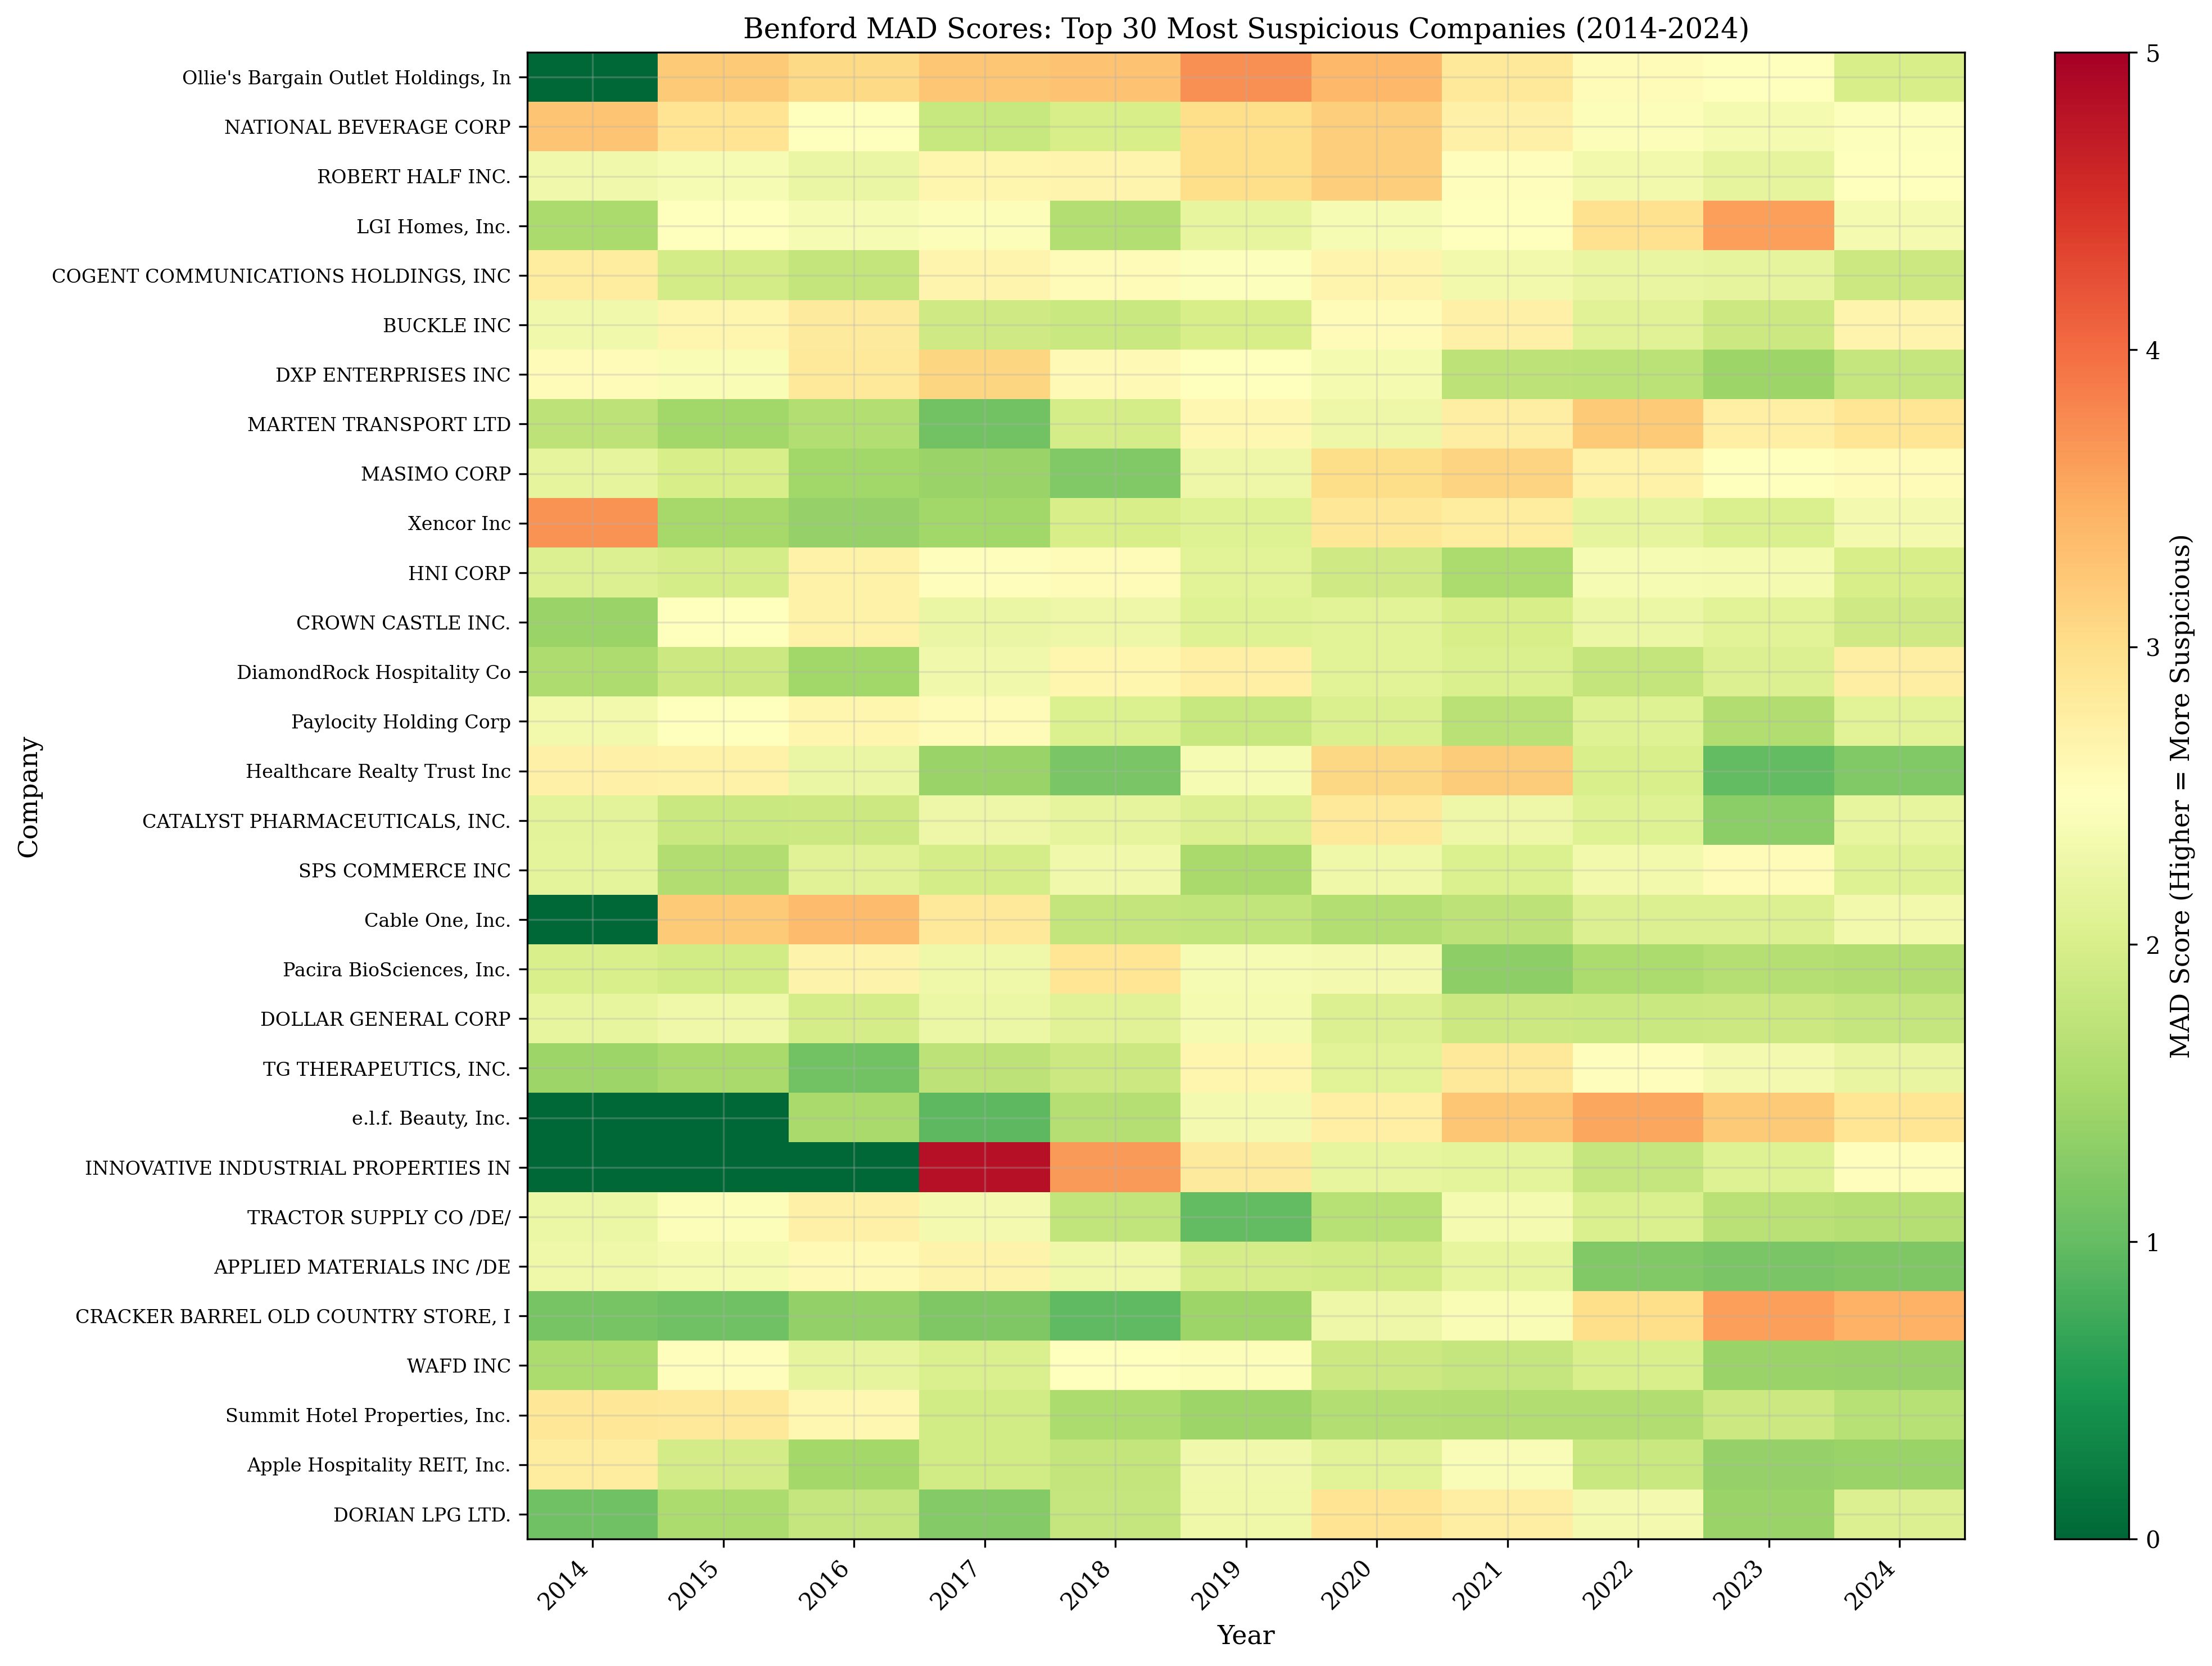
\includegraphics[width=0.95\textwidth]{heatmap_companies.png}
    \caption{Heatmap of MAD scores for the top 30 most suspicious companies (2014--2024). Darker red indicates higher anomaly scores. The vertical banding pattern suggests some year-specific effects across all companies.}
    \label{fig:heatmap}
\end{figure}

Notable patterns:
\begin{itemize}
    \item Vertical bands indicate year-specific effects (e.g., 2018, 2020)
    \item Some companies show consistent elevation across all years
    \item REITs and hospitality companies appear disproportionately represented
\end{itemize}

\newpage
\section{Discussion}

\subsection{Interpretation of Findings}

The high rate of Benford deviation (97.5\%) among S\&P 500 companies is striking but should be interpreted carefully:

\begin{enumerate}
    \item \textbf{Statistical significance $\neq$ practical significance:} With large sample sizes (thousands of line items per company), even minor deviations become statistically significant.

    \item \textbf{Legitimate causes of deviation:} Rounding policies, industry-specific accounting practices, and data aggregation effects can cause non-fraudulent deviations.

    \item \textbf{Benford as screening tool:} High deviation flags companies for further investigation, not automatic fraud determination.
\end{enumerate}

\subsection{Post-2019 Shift}

The 24\% increase in chi-square values after 2019 warrants attention. Potential explanations include:

\begin{itemize}
    \item COVID-19 pandemic introducing unusual accounting estimates
    \item Increased use of fair value measurements under ASC 820
    \item Changes in SEC EDGAR data collection methodology
    \item Greater complexity in revenue recognition (ASC 606 implementation)
\end{itemize}

\subsection{Sector Patterns}

Real Estate Investment Trusts (REITs) and hospitality companies show elevated anomaly rates. This may reflect:
\begin{itemize}
    \item Heavy use of fair value accounting for property valuations
    \item Seasonal revenue patterns creating digit clustering
    \item Industry-specific accounting conventions
\end{itemize}

\subsection{Limitations}

\begin{enumerate}
    \item \textbf{Data granularity:} SEC EDGAR provides aggregated figures; individual transaction data might show better conformance.

    \item \textbf{Sample selection:} Focus on S\&P 500 companies may not generalize to smaller firms.

    \item \textbf{No ground truth:} Without confirmed fraud cases, we cannot validate predictive accuracy.

    \item \textbf{Second-digit analysis:} This study focuses primarily on first-digit tests; second-digit analysis may reveal additional patterns.
\end{enumerate}

\newpage
\section{Conclusion}

\subsection{Summary of Findings}

This thesis analyzed Benford's Law conformance for 442 S\&P 500 companies over 11 years (2014--2024), revealing:

\begin{enumerate}
    \item \textbf{Widespread deviation:} 97.5\% of companies show statistically significant deviation from Benford's expected distribution.

    \item \textbf{Temporal shift:} A 24\% increase in mean chi-square values occurred after 2019, potentially related to COVID-19 and accounting standard changes.

    \item \textbf{Weak market correlation:} Benford anomalies show negligible correlation ($r = 0.03$) with stock returns.

    \item \textbf{Sector effects:} REITs and hospitality companies show systematically higher anomaly rates.

    \item \textbf{Systematic patterns:} Biennial oscillation patterns in 11 companies suggest data structure artifacts rather than fraud.
\end{enumerate}

\subsection{Implications}

For \textbf{auditors and regulators}:
\begin{itemize}
    \item Benford analysis is a useful screening tool but requires contextual interpretation
    \item Industry-specific thresholds may improve accuracy
    \item Automated screening can prioritize limited audit resources
\end{itemize}

For \textbf{investors}:
\begin{itemize}
    \item High Benford anomaly scores alone do not predict poor stock performance
    \item Combined with other signals, anomaly detection may identify accounting quality concerns
\end{itemize}

\subsection{Future Research}

Recommended extensions include:
\begin{enumerate}
    \item Second-digit analysis for detecting rounding manipulation
    \item Machine learning integration for multi-factor anomaly detection
    \item Longitudinal tracking of flagged companies for fraud outcomes
    \item International comparison across different accounting standards
\end{enumerate}

\subsection{Final Remarks}

Benford's Law provides a powerful, objective tool for financial statement analysis. While not a fraud detector per se, it offers valuable insights into data quality and accounting practices. This thesis demonstrates both the utility and limitations of Benford analysis in modern financial forensics.

% References
\newpage
\bibliographystyle{apalike}
\bibliography{references}

\end{document}
